%% 
%% Copyright 2019-2024 Elsevier Ltd
%% 
%% Version 2.4
%% 
%% This file is part of the 'CAS Bundle'.
%% --------------------------------------
%% 
%% It may be distributed under the conditions of the LaTeX Project Public
%% License, either version 1.2 of this license or (at your option) any
%% later version.  The latest version of this license is in
%%    http://www.latex-project.org/lppl.txt
%% and version 1.2 or later is part of all distributions of LaTeX
%% version 1999/12/01 or later.
%% 
%% The list of all files belonging to the 'CAS Bundle' is
%% given in the file `manifest.txt'.
%% 
%% Template article for cas-dc documentclass for 
%% double column output.

%\documentclass[a4paper,fleqn,longmktitle]{cas-dc}
\documentclass[a4paper,fleqn]{cas-dc}

%\usepackage[authoryear,longnamesfirst]{natbib}
%\usepackage[authoryear]{natbib}
\usepackage[numbers]{natbib}
\usepackage[caption=false,font=normalsize,labelfont=sf,textfont=sf]{subfig}
\usepackage{microtype}
\usepackage{amsmath}  % For \max, \mathrm, etc.
\usepackage{bm}       % For bold symbols (optional)
\usepackage{algorithm}
\usepackage{algorithmicx}
\usepackage{algpseudocode}
\usepackage{booktabs}
\usepackage{multirow}
\usepackage{array}   

\setlength{\mathindent}{0pt} % 取消公式的缩进

%%%Author definitions
\def\tsc#1{\csdef{#1}{\textsc{\lowercase{#1}}\xspace}}
\tsc{WGM}
\tsc{QE}
\tsc{EP}
\tsc{PMS}
\tsc{BEC}
\tsc{DE}
%%%

\begin{document}
\let\WriteBookmarks\relax
\def\floatpagepagefraction{1}
\def\textpagefraction{.001}

% Short title
\shorttitle{}    
% Short author
\shortauthors{Pengli Lu et al.}  
% Main title of the paper
\title [mode = title]{Enhanced Metabolite-Disease Associations Prediction via Neighborhood Aggregation Graph Transformer with Kolmogorov-Arnold Networks}  


\author[1]{Pengli Lu}[]
\cormark[1]
\ead{lupengli88@163.com}

\author[1]{Jian Zhang}[]
\ead{jianzhang0934@163.com}

\author[1]{Wenzhi Liu}[]
\ead{lwzvay123@163.com}

\author[2]{Fentang Gao}[]
\ead{gaoft1973@126.com}


%\address[1]{, Street 129, 1043 NX Amsterdam, The Netherlands}
\affiliation[1]{organization={School of Computer and Communication, Lanzhou University of Technology},
	city={Lanzhou}, 
	postcode={730050}, 
	state={Gansu},
	country={China}}

\affiliation[2]{organization={Department of Cardiology, Gansu Provincial People's Hospital},
	city={Lanzhou}, 
	postcode={730000}, 
	state={Gansu},
	country={PR China}}

\cortext[cor1]{Corresponding author}


% Here goes the abstract
\begin{abstract}
Metabolites are essential products of cellular chemical reactions, critical for sustaining life and reproduction.  Research shows that metabolite concentrations in patients differ from those in healthy individuals, making metabolite-based disease prediction crucial for diagnosis and treatment.
To address the limitations of current computational methods in accuracy and interpretability, we propose a novel Neighborhood Aggregation Graph Transformer method (AGKphormer). This method enhances link relationships by optimizing the minimum nuclear norm using the Alternating Direction Method of Multipliers (ADMM) and incorporates Fast Kolmogorov-Arnold Networks (FastKAN) to improve both accuracy and interpretability.
We first construct a heterogeneous network based on the correlation and similarity between metabolites and diseases.  Then, we utilize the ADMM algorithm to enhance link relationships by solving the minimum nuclear norm, reducing sparse relationships between nodes and providing richer features for neural network learning. For the features learned by the graph convolutional network (GCN), we employ a Graph Transformer augmented with FastKAN to learn long-range dependencies. This approach enables global feature embedding and addresses GCN's smoothness issue while enhancing interpretability.
Through five-fold cross-validation, AGKphormer achieved average AUC and AUPR values of 97.32\% and 97.34\%, respectively, outperforming most methods and demonstrating its effectiveness in predicting disease-related metabolites. Additionally, case studies further confirm that AGKphormer is a reliable tool for discovering potential metabolites.
\end{abstract}

% Keywords
% Each keyword is seperated by \sep
\begin{keywords}
	Disease-metabolite associations \sep Graph convolutional networks \sep Graph Transformer \sep Fast Kolmogorov-Arnold Networks
\end{keywords}

\maketitle

% Main text
\section{Introduction}\label{sec1}
Metabolites have a complex and multidimensional relationship with diseases, serving a vital function in maintaining the balance and health of the body's internal environment\cite{transport1}. Metabolites are the products of chemical reactions that occur within cells and are involved in key processes such as cell growth, differentiation, functional maintenance, and immune responses. Imbalances or disorders in metabolic regulation are associated with a variety of diseases, including diabetes\cite{dhanya2016salivary}, obesity\cite{drucker2021diabetes}, cardiovascular\cite{amiri2022role} diseases, and fatty liver diseases. For instance, metabolic abnormalities are considered the root cause of the connection between diabetes and liver diseases. Insulin resistance\cite{lee2022insulin}, diabetes, obesity, and fatty liver are closely linked to liver fibrosis, cirrhosis,  and liver cancer\cite{liu2021transition}.

In disease research, metabolomics helps to reveal the molecular mechanisms between metabolite levels and disease risk\cite{chen2022guide}. Studies have found that genetic variations that regulate metabolite levels may affect gene expression and disease risk. Metabolic diseases are conditions caused\cite{hoffman2021developmental} by genetic mutations or environmental disruptions affecting major digestive organs or organs with significant metabolic functions, such as the liver and pancreas. Disruptions in metabolic pathways can lead to a variety of metabolic diseases, including acid-base imbalances, metabolic brain diseases\cite{jensen2020effects}, and lipid metabolic disorders\cite{aron2021metabolism}. The role of metabolism is also an increasingly important aspect in cancer research. Cancer cells rely on inefficient fermentative metabolic pathways, a phenomenon known as the "Warburg effect"\cite{vaupel2021revisiting} which is a hallmark of many cancers and reflects the metabolic adaptations that promote cancer cell growth and survival. Cancer cells require their nutrient inputs as the basic components of the cell, shifting from catabolic pathways to anabolic pathways to support their high proliferation rates\cite{martinez2021cancer}. Therefore, there is a close connection between metabolites and diseases, and a deep understanding of these connections is of great significance for the prevention, diagnosis, and treatment of diseases.

Traditional wet experiments are inefficient for detecting the relationship between diseases and metabolites. With the advancement of metabolomics and data mining techniques, multiple databases dedicated to studying metabolomics have been established, including METLIN\cite{montenegro2020metlin}, HMDB\cite{wishart2022hmdb}, and gutMGene\cite{cheng2022gutmgene}. Along with this, there are methods for computationally identifying the relationship between metabolites and diseases, which can avoid the shortcomings of traditional experiments. The development of machine learning has given rise to approaches that primarily utilize optimization and complex network algorithms.
In 2018, Hu et al. used random walk to identify diseaserelated metabolites\cite{hu2018identifying}. Later, Lei et al. developed a calculation method based on KATZ to predict the metabolite–disease associations\cite{lei2019predicting}. This is also the first application of KATZ algorithm in the field of metabolomics. In 2020, Lei et al. proposed a linear neighborhood similarity with improved bipartite network projection algorithm to predict associations between metabolites and diseases\cite{lei2020predicting}. Furthermore, Zhao et al. introduced a Deep-DRM model in 2021\cite{zhao2021deep}, employing graph convolution networks and principal component analysis (PCA) for identifying metabolite–disease associations. In the same year, Zhang et al.proposed LGBMMDA\cite{zhang2021predicting}, a method that extracts features from various measurements, applies PCA for noise reduction and utilizes the LGBM classifier for analysis. In 2022, Tie et al. proposed a metabolite–disease association prediction algorithm based on DeepWalk and random forest\cite{tie2021metabolite}. During the same period, Sun et al. came up with a graph neural network with attention mechanisms to predict the associations between metabolites and diseases\cite{sun2022deep}. In 2023, Gao et al. proposed a method for predicting metabolite-disease associations based on autoencoders and non-negative matrix factorization\cite{gao2023predicting}. Despite the achievements of current predictive models, there are still some limitations.

Compared to general computational methods, the development of deep learning has greatly improved computational efficiency.
However, the core idea of existing graph neural networks (GNNs) is to propagate and aggregate information through adjacency matrices to learn complex representations of graphs. 
However, the currently constructed association networks are overly sparse, with known associations accounting for only 0.77\%. This may lead to problems such as information loss, decreased accuracy, and difficulty in capturing complex patterns, which makes the exploration of node information not deep enough and limits the performance of the model. With in-depth research on the GCN architecture\cite{kipf2017semisupervisedclassificationgraphconvolutional}, its drawbacks have become increasingly apparent. Although it performs well in processing graph-structured data, traditional GCN models may encounter problems such as gradient vanishing and over-smoothing, which make it difficult for the model to distinguish different nodes, thus affecting performance.
In addition, research and application of Transformers\cite{vaswani2023attentionneed} are rapidly developing, and in recent years, they have achieved performance comparable to or better than the most advanced GNN models in graph-related tasks. Compared to traditional GNN, they can handle long-range dependencies and complex topological structures in graphs. However, due to high computational complexity, poor generalization ability, and low interpretability, they still require more optimization and improvement in practical applications. This will drive our work forward.

Inspired by the aforementioned issues, we propose AGKphormer, which employs the ADMM algorithm optimization algorithm to minimize the nuclear norm for enhancing association relationships, and then uses a model based on GCN and integrates FastKAN in a Transformer model to further deduce the relevance between metabolites and diseases. 
Firstly, we constructed a heterogeneous network based on known association intelligence and the similarity networks of diseases and metabolites. Next, we use the ADMM\cite{MAL-016} optimization algorithm to solve for the minimum nuclear norm on the heterogeneous network to enhance the known link relationships, which will supplement the sparse associations between diseases and metabolites, thereby improving accuracy.
Then, we use the constructed graph neural network to extract feature from the input graph structural data. We find that the message passing mechanism of GCN helps to integrate representations and graph structures. 
The Transformer can directly establish connections between any two positions in the sequence, effectively capturing long-range dependencies. 
Combining the two will capture more topological information of the graph, and we utilize FastKAN within the Transformer to enhance its accuracy and interpretability. 
Finally, a bilinear decoder is used to reconstruct the association network between diseases and metabolites. The following summarizes the three main contributions of this research.
\begin{itemize}
	\item For the first time, we employ a method based on the ADMM algorithm to minimize the nuclear norm to enhance the sparse disease-metabolite associations, thereby providing additional features for subsequent neural network learning.
	
	\item By combining GCN with a Graph Transformer, we developed a neural network for global feature learning, thereby enhancing the overall performance of the model.
	
	\item We improved the optimization of the Graph Transformer by introducing the more interpretable FastKAN, thereby enhancing the performance and interpretability of the model's learning process.
	
	\item We propose a novel graph neural network, AGKphormer, based on enhanced link relationships, which inherits the advantages of traditional graph neural networks and Transformers, while also introducing the new FastKAN to enable more comprehensive and in-depth mining of feature information.
\end{itemize}

We evaluated the performance of AGKphormer in a 5-fold cross-validation experiment, and the results outperformed five existing computational methods. Additionally, we conducted case analyses based on AGKphormer and found that most of the top 15 predicted metabolite-disease associations are verifiable in relevant literature. These results indicate that AGKphormer is an effective and accurate model for predicting metabolites with potential associations to diseases.


\section{Preliminaries}\label{sec2}
In this section, the concepts of relevant databases, known associations, and similarity calculations are mainly introduced, which will be utilized in the subsequent work.

\subsection{Dataset}
HMDB (Human Metabolome Database, \url{https://hmdb.ca/})\cite{wishart2022hmdb} is a widely used biochemical database that focuses on storing information related to human metabolism. 
We extracted a dataset from version 5.0 of HMDB that includes disease IDs (DOID) and related metabolite information. After removing noise from the raw data, we cleaned and filtered it to obtain 657 diseases, 2,624 metabolites, and 7,772 detected and quantified associations. Additionally, diseases and metabolites were uniformly named using MeSH Unique ID (Medical Subject Headings)\cite{lipscomb2000medical} and HMDB ID, resulting in Dataset 1 which comprises 265 diseases, 2,315 metabolites, and 4,763 associations. 
Additionally, we compiled Dataset 2 based on Zhao et al.'s \cite{zhao2021deep} research by removing diseases lacking MeSH Unique IDs and their corresponding associations, thereby further validating the model's generalization capability. The dataset comprises 126 diseases, 1,405 metabolites, and 2,555 documented associations.

\subsection{Metabolite–disease associations}
To delve into the interplay between diseases and metabolites, we constructed an adjacency matrix $A = (a_{i,j})_{N_{m}*N_{d}}$ to quantify their Associations. In this matrix, $ N_{m}$ and $N_{d} $ denote the number of metabolites and diseases. Specifically, if there is a known scientific association between disease \(i\) and metabolite \(j\), then the element $a_{ij}$ in matrix \(A\) is marked as \(1\), conversely, if there is no direct connection between the two, $a_{ij}$ is 0.


\subsection{Similarity measures}
\subsubsection{Disease semantic similarity}
Disease semantic similarity \cite{wang2010inferring} can be calculated based on disease information from the MeSH database. Based on the topological structure of the disease ontology and the hierarchical relationships between diseases, an information content contribution factor is introduced. The relationships between diseases can be represented as \(DAG(d) = (d, T(d), E(d))\), where \( T(d) \) denotes \( d \) itself and all the ancestor nodes of \( d \), and \( E(d) \) represents the set of directed edges from the ancestor nodes to the disease nodes. The semantic value of the disease \( DV(d) \) can be defined as:
\begin{equation}
DV(d) = \sum_{n \in T(d)} D_d(n)
\end{equation}
where \(T(d)\) denotes the set of disease \(d\) and its ancestor nodes, and \( D_d(n)\) represents the semantic contribution value of disease \(n\) to \(d\), \( D_d(n) \), is defined as follows:\\
\begin{equation}
	D_{d}(n) = 
	\begin{cases}
		1, & n = d \\
		\max\bigl\{\Delta \cdot D_{d}(n') \mid n' \in \text{children of } d\bigr\}, & n \neq d
	\end{cases}
\end{equation}
Where \(\Delta\) is defined as a decay factor of 0.5, and the semantic contribution value is inversely proportional to the distance between diseases. The semantic similarity of diseases $d_i$ and $d_j$ is defined below:
\begin{equation}
	DSS(d_i, d_j) = \frac{\sum_{t \in T(i) \cap T(j)} \left(D_i(t) + D_j(t)\right)}{DV(i) + DV(j)}
\end{equation}

\subsubsection{Gaussian kernel similarity for disease and metabolite}
The Gaussian kernel\cite{ter2003gaussian} is used to measure the similarity or distance between data points. Using known topological information from the disease-metabolite association network, kernel methods are employed to construct a kernel function from feature vectors in order to extract associated features. The Gaussian kernel similarity network\cite{van2011gaussian} of diseases and metabolites can be calculated as follows:
\begin{equation}
	\operatorname{DGS}(d_{i}, d_{j})=\exp\left(-\omega_{d}\left\|\operatorname{IP}(d_{i})-\operatorname{IP}(d_{j})\right\|^{2}\right)
\end{equation}
\begin{equation}
	\operatorname{MGS}(m_{i}, m_{j})=\exp\left(-\omega_{m}\left\|\operatorname{IP}(m_{i})-\operatorname{IP}(m_{j})\right\|^{2}\right)
\end{equation}
where IP ($d_{i}$) and  IP($d_{j}$) represent the feature mappings of dieases $d_{i}$ and $d_{j}$, and IP ($m_{i}$) and  IP($m_{j}$) represent the feature mappings of metabolites $m_{i}$ and $m_{j}$, 
$\omega_{d}^{\prime}$ and $\omega_{m}^{\prime}$ is a weight parameter that regularizes the influence of distance in the similarity measure. Here, the weight parameters are set to 1, and the calculations are as shown in Equations (6) and (7):
\begin{equation}
	\omega_{d} = \omega_{d}^{\prime} / \left(\frac{1}{n_{d}} \sum_{i=1}^{n_{d}} \operatorname{IP}(d_{i})^{2}\right)
\end{equation}
\begin{equation}
	\omega_{m} = \omega_{m}^{\prime} / \left(\frac{1}{n_{m}} \sum_{i=1}^{n_{m}} \operatorname{IP}(m_{i})^{2}\right)
\end{equation}


\subsubsection{Metabolite molecular fingerprint similarity}
Metabolite molecular fingerprint similarity\cite{gao2023predicting} refers to the assessment of structural similarity between different metabolite molecules by comparing their fingerprints in the context of metabolomics research. A molecular fingerprint is an encoding method that represents the molecular structure. We convert the collected chemical structures in SMILES format into a set of binary molecular fingerprints. Thereafter, the Tanimoto coefficient\cite{lim2016large,willett1998chemical} is utilized to quantify the differences between various metabolites. The specific formula is as follows:
\begin{equation}
	MFS(m_{i}, m_{j}) = \frac{\gamma}{\alpha + \beta - \gamma}
\end{equation}
where \( \alpha \) and \( \beta \) represent the number of occurrences of 1 in the molecular fingerprints of metabolites \( m_{i} \) and \( m_{j} \), respectively, and \( \gamma \) indicates the number of common occurrences of 1 in both metabolite \( m_{i} \) and \( m_{j} \).


\begin{figure*}[htbp]
	\centering
	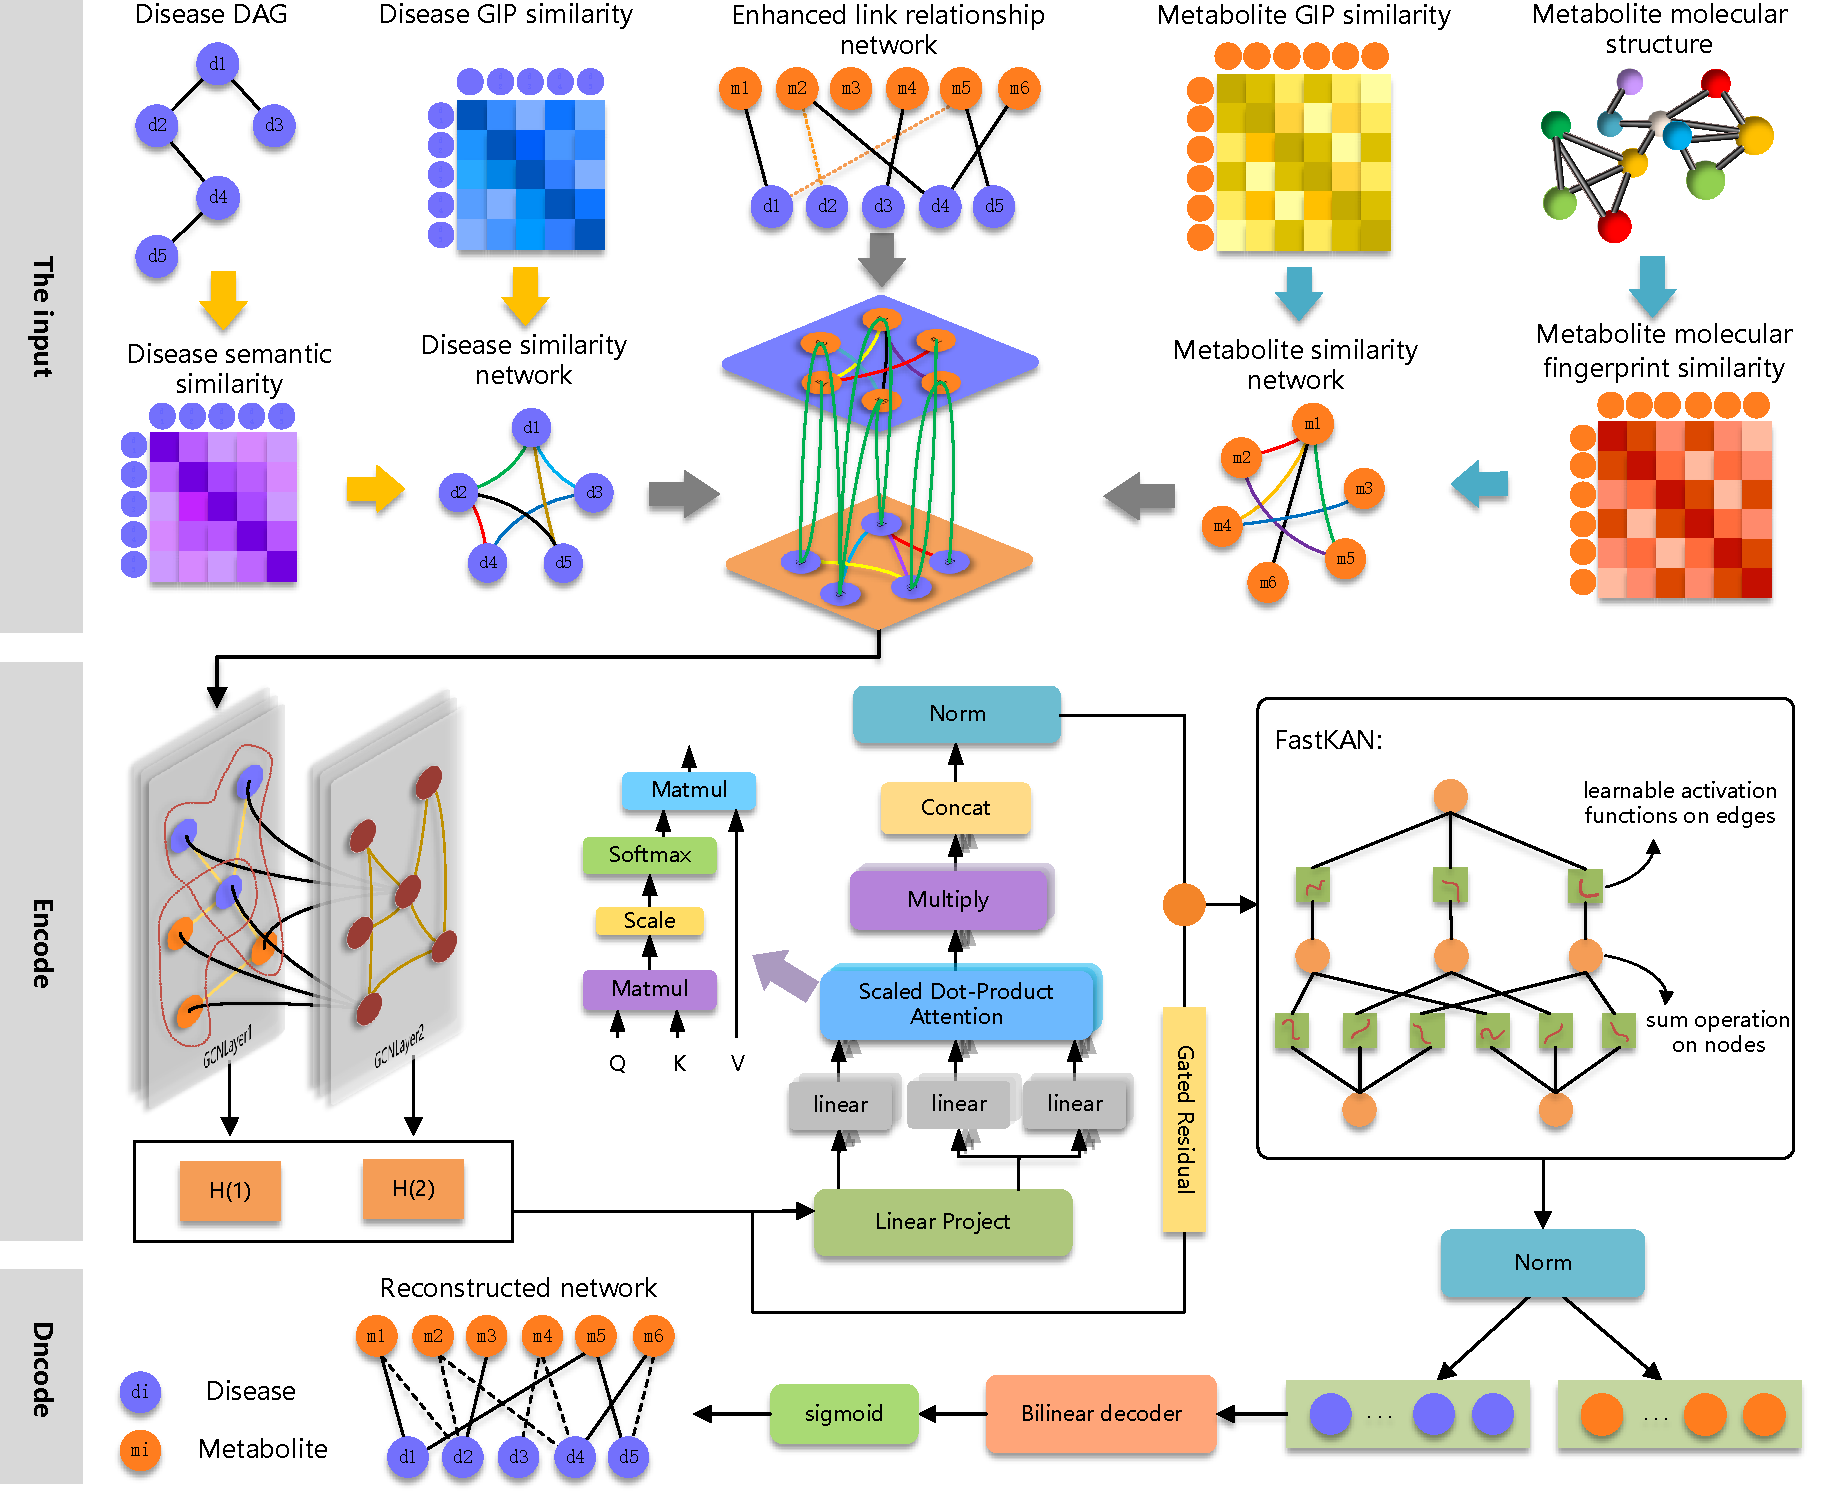
\includegraphics[width=17cm]{flow_chart_05.3.pdf}
	\caption{Overall flow chart of the AGKphormer mode.}
	\vspace{-3mm} %调整纵向距离
	\label{fig1}
\end{figure*}


\section{Methdos}
The overall workflow of AGKphormer is illustrated in Fig.\ref{fig1}, consisting of four steps. The model proposed in this paper is divided into four steps. First, we construct the disease similarity matrix NSD and the metabolite similarity matrix MSN using similarity measures. Next, we enhance the known associations between metabolites and diseases based on the ADMM optimization method that minimizes the nuclear norm. Then, we construct a heterogeneous network based on the enhanced association matrix and the similarity matrices DSN and MSN. Subsequently, we feed this heterogeneous network as input into the Graph Convolutional Network (GCN), where the GCN encoder is used for neighborhood feature learning. These learned features are then input into our improved Transformer encoder, which consists of Multi-Head Attention and FastKAN, utilizing residual connections to enhance training efficiency. This encoder is more effective at modeling long-range dependencies between nodes in the graph and can learn node representations from multiple subspaces. Finally, a bilinear decoder is used to decode the obtained metabolite-disease embeddings to reconstruct the metabolite-disease association matrix, thereby inferring potential metabolite-disease relationships.


\subsection{Construct disease and metabolite similarity networks}
To address the issue of zero semantic similarity, we will integrate the Gaussian kernel similarity of diseases to construct a comprehensive similarity matrix DSN. This approach helps to mitigate the situation by providing an alternative measure of similarity that does not rely solely on semantic descriptions, thereby enhancing the robustness of the similarity assessment.
\begin{equation}
	\operatorname{DSN}(d_i, d_j) = \begin{cases} 
		\operatorname{DGS}(d_i, d_j), & \operatorname{DSS}(d_i, d_j) = 0 \\
		\frac{\operatorname{DGS}(d_i, d_j) + \operatorname{DSS}(d_i, d_j)}{2}, & \text{otherwise}
	\end{cases}
\end{equation}
Similarly, for metabolites, there are cases where metabolites do not have corresponding molecular fingerprint profiles, resulting in a molecular fingerprint similarity of zero. To address this, we combine the Gaussian kernel similarity of metabolites to construct a comprehensive similarity matrix MSN.
\begin{equation}
	\small
	\operatorname{MSN}(m_i, m_j) = \begin{cases} 
		\operatorname{MGS}(m_i, m_j), &\operatorname{MFS}(m_i, m_j)=0 \\
		\frac{\operatorname{MGS}(m_i, m_j) + \operatorname{MFS}(m_i, m_j)}{2}, & \text{otherwise}
	\end{cases}
\end{equation}

As we know, there is no association between disease-disease and metabolite-metabolite, therefore we construct a comprehensive similarity between diseases and metabolites to complement the correlation among nodes of the same type, to better mine the information in the graph, and to better predict potential links.


\subsection{Enhancing Association Links}
After data processing, our final dataset encompasses 2,315 metabolites and 265 diseases, generating 613,475 association pairs, with only 4,764 being known associations. The original association matrix exhibits extreme sparsity and binary discreteness, manifested by known associations constituting 0.77\% (calculated as 4,763 known associations divided by 613,475 total possible associations) and containing only elements 0 and 1. This sparsity renders traditional interpolation-based methods relying on observed values ineffective for recovering underlying association patterns. Leveraging biological priors of metabolite functional similarity and disease phenotypic associations, we propose an ADMM-based nuclear norm minimization framework. The theoretical foundation of this design lies in the multi-target regulatory nature of metabolites, which endows the association matrix with inherent low-rank structure. The nuclear norm (sum of matrix singular values), serving as a convex relaxation of the rank function, precisely characterizes this structure. Meanwhile, under sparse observation conditions, the nuclear norm constraint enables more stable matrix completion by suppressing high-dimensional noise subspaces. This process is illustrated in Fig.\ref{fig2}.

\begin{figure}[htbp]
	\centering
	\vspace{-3mm} %调整纵向距离
	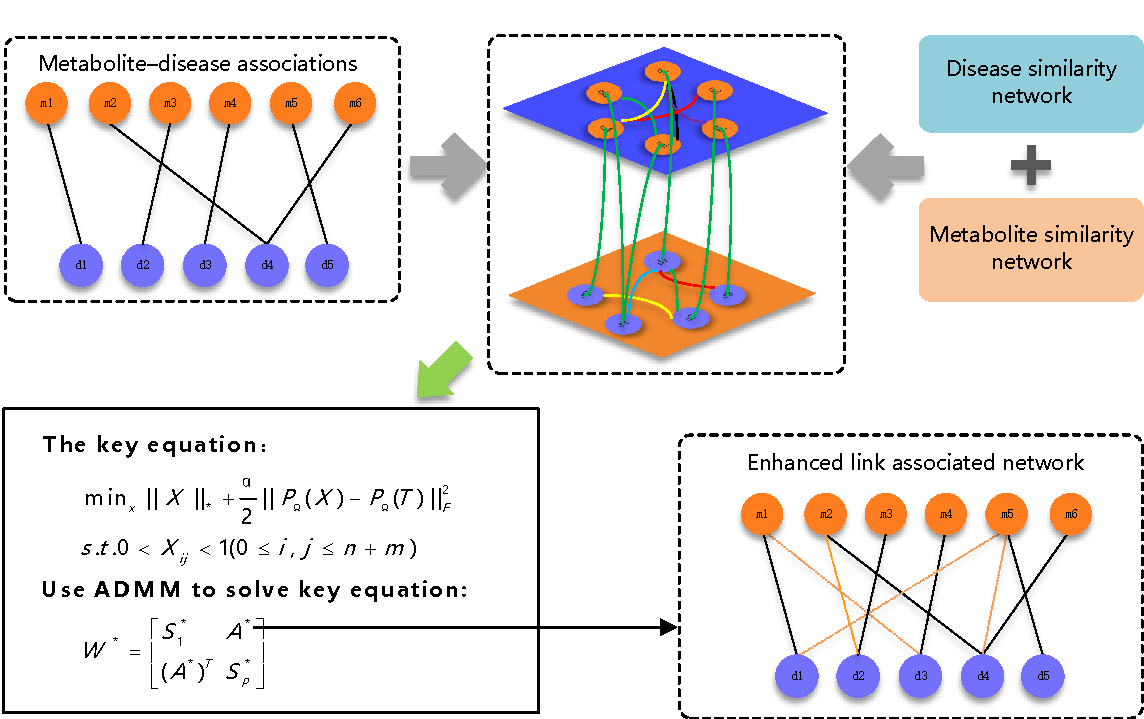
\includegraphics[width=8cm]{ADMM_flow_02.pdf}
	\caption{Overview of Methods for Matrix Completion.}  % with Minimum Nuclear Norm
	\vspace{-3mm} %调整纵向距离
	\label{fig2}
\end{figure}


\subsubsection{Construct the target matrix}
To avoid issues caused by the sparsity of the matrix, such as a decrease in prediction accuracy, this paper enhances the associations by minimizing the nuclear norm. First, based on the previously constructed similarity networks and the metabolite-disease interaction adjacency matrix, a heterogeneous metabolite-disease network T is built as our target matrix, represented as follows:
\begin{equation}
	T = \begin{bmatrix} MSN & A \\ A^T & DSN \end{bmatrix}	
\end{equation}


It is not difficult to deduce that the target matrix \( T \) is of dimension \( (n+m) \times (n+m) \), that is, \( 2315 \times 2315 \) in size.

\subsubsection{Complete the matrix}
After constructing the target matrix T, we fill the missing values using the computed metabolite-disease prediction scores. Since metabolite-disease association patterns typically exhibit low-rank properties, we transform the matrix completion problem into a low-rank matrix optimization problem\cite{ramlatchan2018survey}, which can also be a problem of minimizing the matrix's nuclear norm\cite{candes2013simple}. During this process, we found that the ADMM algorithm\cite{MAL-016} not only has fast decomposition speed but also achieves good performance in terms of "slimming down" the matrix. Therefore, we ultimately transform the problem into:
\begin{equation}
	min_X \|X\|_*  \;\;\;\;\;   \text{s.t.}\!\!\!\!\quad P_\Omega(X) = P_\Omega(T)
\end{equation}
where \(\|X\|_*\) represents the nuclear norm of \( X \), \( \Omega \) is the set of coordinates of the target matrix nodes, corresponding to the known metabolite-disease pairs.  \( P_\Omega \) is the orthogonal projection operator on \( \Omega \).
\begin{equation}
	\left(P_{\Omega}(X)\right)_{ij} = \begin{cases} 
		X_{ij}, & (i, j) \in \Omega \\
		0, & \text{otherwise}
	\end{cases}
\end{equation}

In addition, to further enhance the ADMM algorithm, we have included a regularization term and matrix value constraints in the equation. Furthermore, we have introduced a weight matrix \( W \) in the function to improve convergence performance. The key objective equation is obtained as follows:
\begin{equation}
	\begin{split}
		\min_X & \|X\| + \frac{\alpha}{2} \left\| P_{\Omega}(W) - P_{\Omega}(T) \right\|_F^2 \\
		\text{s.t.} & \quad X = W, \quad 0 < W_{ij} < 1 \quad (0 \leq i, j \leq n+m)
	\end{split}
\end{equation}

where \( \alpha \) is the parameter characterizing the error term, \( 0 \leq X_{ij} \leq 1 \) represents that all elements in \( X \) are within the range (0, 1). \( W \) is the auxiliary matrix. The Augmented Lagrangian function is:
\begin{equation}
	\begin{split}
		L(W, X, Y, \alpha, \beta) = 
		 \|X\|_* + \frac{\alpha}{2} \left\| P_{\Omega}(W) - P_{\Omega}(T) \right\|_F^2  \\
		+ \text{Tr}(Y^T (X - W)) +\frac{\beta}{2} \|X - W\|_F^2
	\end{split}
\end{equation}
where \( Y \) is the Lagrange multiplier, \(alpha\) represents the nuclear norm weight, \( \beta > 0 \) represents the penalty parameter. We initialize \( W \), \( X \), and \( Y \) to \( P_{\Omega}(T) \), and then perform iterations. 
The iterative procedure of the ADMM optimization algorithm is presented in Algorithm.\ref{admm} , First, \(W\) preserves known values while estimating unknowns via \(X-Y/\beta \), next, \(X\) is obtained by thresholding singular values of \(W+Y/\beta \), finally \(Y\) adjusts based on the \(W-X\) discrepancy. Iterations continue until \(||W-X||_F\) converges or maximum iterations are reached, yielding the completed matrix. 
When the iteration terminates, the final prediction matrix \( W^* \) can be obtained, where \( A^* \) represents the enhanced metabolite-disease association matrix. The prediction matrix and the termination conditions for the iteration are as follows:
\begin{equation}
	\begin{split}
		& W^* = \begin{bmatrix} MSN^* & A^* \\ {A^*}^T & DSN^* \end{bmatrix} \\
		& d1_{k+1} = \frac{\left\| X_{k+1} - X_k \right\|_F}{\left\| X_k \right\|_F} \leq \text{tol}_1 , \\
		& d2_{k+1} = \frac{\left| d1_{k+1} - d1_{k} \right|}{\max\left\{ \left| d1_{k} \right|, 1 \right\}} \leq \text{tol}_2
	\end{split}
\end{equation}

\begin{algorithm}[H]
	\caption{ADMM for Matrix Completion}
	\label{admm}
	\begin{algorithmic}[1]
		\Require Observed matrix $M$, mask $P_\Omega$, parameters $\rho$, $\alpha$, $\mathrm{max\_iter}$
		\Ensure Completed matrix $W$
		\State Initialize: $W \gets P_\Omega(M)$, $X \gets \mathbf{0}$, $Y \gets \mathbf{0}$
		\For{$k = 1$ to $\mathrm{max\_iter}$}
		\State $W \gets P_\Omega(M) + (X - Y/\rho) \odot (1 - P_\Omega)$
		\State $[U,S,V] \gets \mathrm{svd}(W + Y/\rho)$
		\State $X \gets U \cdot \mathrm{diag}(\max(S - 1/\rho, 0)) \cdot V^\top$ 
		\State $Y \gets Y + \rho(W - X)$ 
		\If{$\|W - X\|_F < \mathrm{tol}$}
		\State \textbf{break}
		\EndIf
		\EndFor
		\State \Return $W$
	\end{algorithmic}
\end{algorithm}
Finally, we extract the submatrix \(A^*\) from the upper-right quadrant of the \(W^*\) matrix as the enhanced metabolite-disease association matrix, which will be used for subsequent graph construction and model learning.

\subsection{Graph Encoder}
Building upon strengthened associations, we designed a novel graph encoder architecture. To address the local topological structures inherent in the original heterogeneous network, the Graph Convolutional Network (GCN) layer performs neighborhood aggregation to effectively capture first-order node proximity, generating node embeddings with local structural awareness. These embeddings are then processed through multi-head attention mechanisms to capture global node interactions, thereby mitigating the over-smoothing problem commonly observed in GCNs. Finally, FastKAN is employed to enhance the model's capability in learning complex nonlinear relationships within metabolic pathways. This hierarchical design establishes a comprehensive feature learning pipeline that simultaneously preserves both local and global topological characteristics while improving model interpretability.

\subsubsection{Neighborhood Feature Aggregation}
GCN\cite{kipf2017semisupervisedclassificationgraphconvolutional}, as a type of graph neural network, is based on the core idea of aggregating the feature information of neighboring nodes and then learning from it through a neural network. First, the newly constructed heterogeneous network \(G\) is standardized to obtain \( \tilde{G} \), which is typically achieved by multiplying the inverse of the degree matrix \( D \) with its square root, that is:
\begin{equation}
	\tilde{G} = D^{-\frac{1}{2}} G D^{-\frac{1}{2}}.
\end{equation}
Next, the standardized adjacency matrix \( \tilde{G} \) is multiplied with the node feature matrix \( X \) to achieve the aggregation of feature information.Finally, the learned weight matrix W is multiplied with the aggregated features through matrix multiplication to obtain the new node feature representation. The GCN can be expressed by the following formula:
\begin{equation}
	H^{(l+1)} = D^{-\frac{1}{2}} G D^{-\frac{1}{2}} H^{(l)} W
\end{equation}
where \( H^{(l)} \) is the embedding of the nodes at layer \( L \), and \( W \) is the layer-specific trainable weight matrix.To better utilize the similarity characteristics, we set the input adjacency matrix to be:
\begin{equation}
	G = \begin{bmatrix} MSN & A^* \\ {A^*}^T & DSN \end{bmatrix}	
\end{equation}
G is constructed from the integrated similarity matrices MSN and DSN of metabolites and diseases, along with the completed adjacency matrix \(A^*\) obtained through our matrix completion process. We then initialize the feature matrix as:
\begin{equation}
	X = \begin{bmatrix} 0 & A \\ A^T & 0 \end{bmatrix}	
\end{equation}

Finally, according to the formula, we learn from the input graph to obtain a new feature matrix as subsequent input.

\subsubsection{Multi-Head Attention}
Here, we have implemented the multi-head attention\cite{cordonnier2020multi} mechanism using a graph transformer\cite{shi2021maskedlabelpredictionunified}, serving as a message-passing neural network layer capable of learning and capturing long-range dependencies. Specifically, for the node features \(H \in \mathbb{R}^{n \times d} \) after graph convolution,We use learnable weights to compute the queries, keys, and values corresponding to each node feature \( h_i \), respectively:
\begin{equation}
	Q_i = W_qh_i, \ K_i = W_kh_i, \ V_i = W_vh_i, 
\end{equation}

then divide the transformed results into multiple heads. For each head, we calculate the dot product of \( q_i \) and \( k_j \), then divide by a scaling factor to obtain the unnormalized attention scores. Then, normalize the attention scores using the softmax function\cite{liu2017largemarginsoftmaxlossconvolutional} to obtain the attention weights:
\begin{equation}
	\alpha_{i,j} = softmax(\frac{{Q}_i^\top {K}_j}{\sqrt{d_k}})
\end{equation}
where \( d_k \) represents the dimension of the key vector. 

Multiply the normalized attention weights by their corresponding values \({v}_j\), and sum over all nodes to obtain the aggregated features:
\begin{equation}
	{x}_i = \sum_{j \in {N}_{(i)}} \alpha_{i,j} {V}_j
\end{equation}
where \({N}_{(i)}\) is the representation of the neighbors of node \(i\),
then, we use concatenation to join the outputs of all heads:
\begin{equation}
	{m}_i = \text{Concat}({x}_i^1, {x}_i^2, ..., {x}_i^H)
\end{equation}
Additionally, we employ residual connections\cite{szegedy2017inception} to combine the original node features with the aggregated features, addressing the issue of vanishing gradients:
\begin{equation}
	{h}_i' = {W}_o {h}_i + {m}_i
\end{equation}
where \({W}_o\) is the learnable weight matrix. In the end, the output feature \({h}_i'\) of node \(i\) is a combination of the aggregated features and the skip connection.
In summary, based on the above formulas, for the GCN output features \( H \), the multi-head attention captures deeper embedding information, and the final output features are:
\begin{equation}
	x_{i}^{\prime} = W_{o}x_{i} + \sum_{j \in {N}_(i)} \operatorname{softmax}\left(\frac{\left(W_{q} x_{i}\right)^{\top}\left(W_{k} x_{j}\right)}{\sqrt{d_{k}}}\right)W_{v}x_{j}
\end{equation}

\subsubsection{FastKAN}
To enhance nonlinearity and increase the model's expressive power, as well as to help the model understand the global and local structures in the data, we introduce FastKAN\cite{li2024kolmogorovarnoldnetworksradialbasis}, which provides greater interpretability for the model.

Unlike traditional Multi-Layer Perceptrons (MLP)\cite{taud2018multilayer}, the core idea of KAN\cite{liu2024kankolmogorovarnoldnetworks} is to replace each weight parameter with a learnable univariate function, usually a parameterized spline function, thus the entire network contains no linear weights. Specifically, KAN represents the function \( f(x) \) as:
\begin{equation}
	f(\mathbf{x}) = \sum_q \Phi_q \left( \sum_p \phi_{q,p}(x_p) \right)
\end{equation} 
where \( \Phi \) and \( \Phi_{q,p} \) are univariate functions.
The design of KAN allows it to break down complex functions into simpler components for easier understanding. It uses B-splines to construct a family of functions that effectively approximate smooth univariate functions. However, if variables exceed the set neighborhood during training, adjustments to the spline grid are needed, requiring recalculation of the B-spline\cite{de1972calculating} basis through deBoor-Cox iteration, which may lead to efficiency bottlenecks.

To enhance efficiency while ensuring accuracy, we have implemented FastKAN as a replacement for traditional methods. FastKAN utilizes Gaussian kernel radial basis functions (RBFs)\cite{buhmann2000radial} to approximate third-order B-spline bases and applies layer normalization to prevent input data from exceeding the RBF range.
This can be expressed as follows:
\begin{equation}
	f(x) = \sum_{i=1}^{N} w_{i} \phi\left( \left\| x - c_{i} \right\| \right)
\end{equation}
where \( w_i \) is the learnable weight, \(\| x - c_i \|\) represents the distance between the input \(x\) and the center \(c_i\). The radial basis function (RBF) we use is:
\begin{equation}
	\phi( \left\| x - c_{i} \right\|) = \exp\left(-\frac{ \left\| x - c_{i} \right\|^2}{2h^2}\right)
\end{equation}
where \(h\) is a parameter used to control the width of the function.

Specifically, for the features we learned earlier, we apply layer normalization, then generate high-dimensional features through RBF, and next, flatten the high-dimensional features generated by RBF and use the spline linear layer to map them to the output dimensions. Finally, after processing the original input features through an activation function and linearly mapping them, we add them to the output of the RBF features to obtain the output of the generated layer. This will further help us extract feature information.

This design not only improves computational efficiency but also offers two major advantages compared to the fixed activation functions and linear combinations in traditional MLPs. First, the learnable radial basis term can adaptively capture node features. Second, the use of third-order spline basis ensures smoothness constraints during feature propagation while enhancing the model's interpretability through explainable function decomposition.

\subsection{Decoder}
After encoding the node features through our encoder to capture global and long-range structural information, we obtain the final embeddings for metabolites and diseases. Subsequently, we decode the final output to obtain the association probabilities between metabolites and diseases, resulting in the final association matrix:
\begin{equation}
	H^{(2)} = \begin{bmatrix} {H_m}^{(2)}  \\ {H_d}^{(2)} \end{bmatrix}	
\end{equation}
\begin{equation}
	A' = sigmod \left({H_m}^{(2)} W  {({H_d}^{(2)})}^T \right)
\end{equation}
where \( H^{(2)}_m \in \mathbb{R}^{2315 \times 512} \) and \( H^{(2)}_d \in \mathbb{R}^{265 \times 512} \) are the final embeddings of the diseases and metabolites, and \( W \in \mathbb{R}^{512 \times 512} \) is the trainable weight.

Additionally, we chose the cross-entropy loss function \cite{mao2023cross} as the loss function for the model:
\begin{equation}
	L = -y \log(\hat{y}) - (1 - y) \log(1 - \hat{y})
\end{equation}

Meanwhile, the Adam optimizer \cite{kingma2014adam} is used to update parameters, thereby accelerating the model's convergence. To prevent overfitting, dropout\cite{baldi2013understanding} is also used during the encoding process, with the aim of training different subnetworks in different batches.





%--------------------------------------------------------------------------------------------------------------
\section{Result}
\subsection{Evaluation indexes}

\begin{figure*}[htbp]
	\centering
	\vspace{-1mm} %调整纵向距离
	\begin{tabular}{cc}
		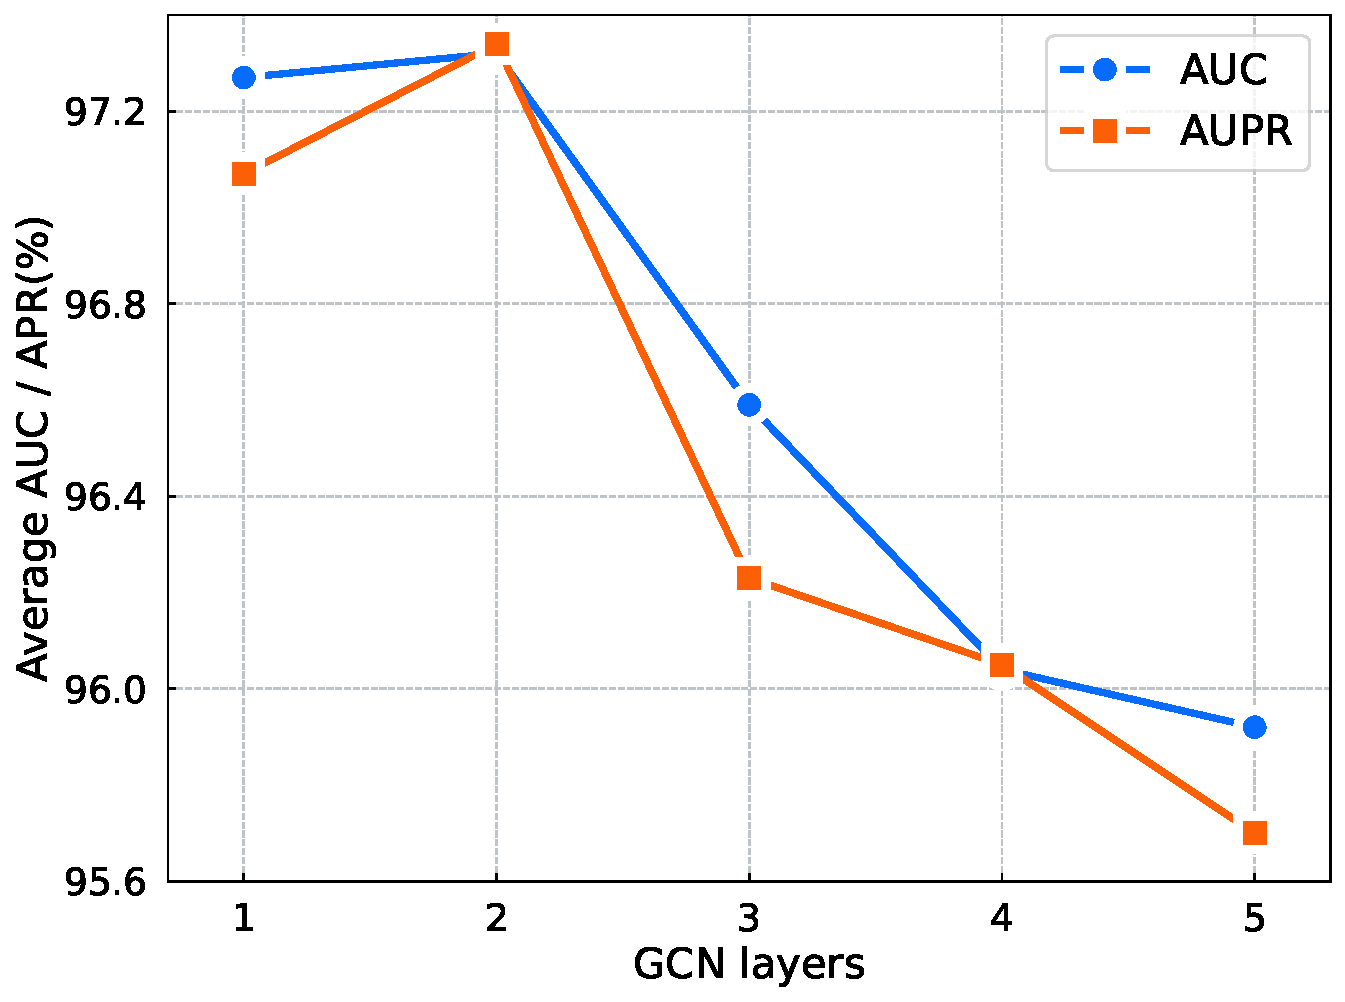
\includegraphics[width=3in]{GCN_layer.pdf} &
		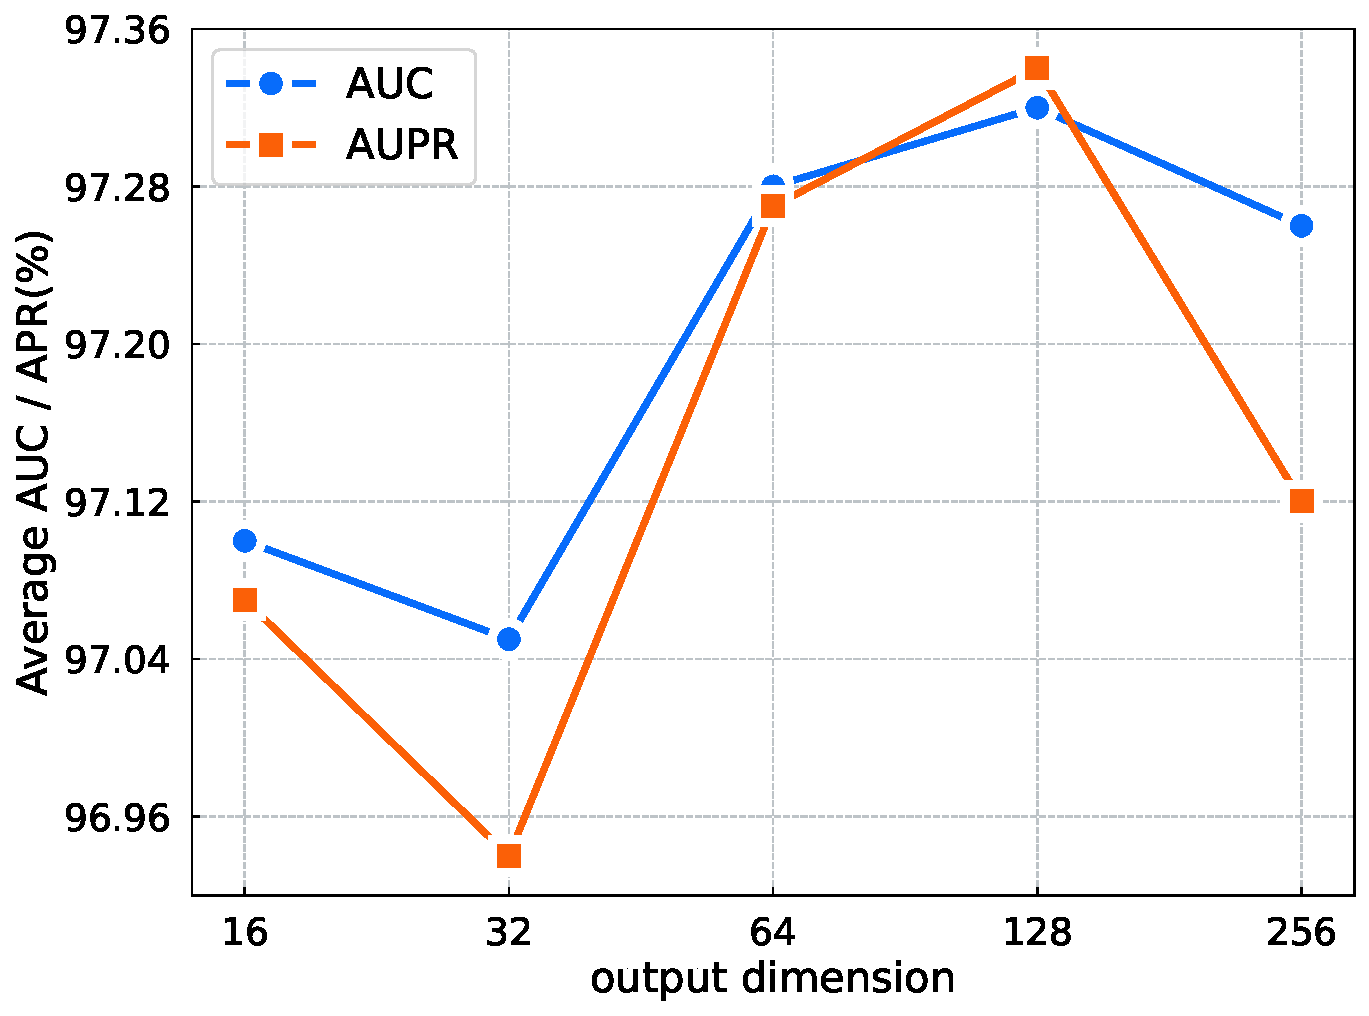
\includegraphics[width=3in]{out_dim.pdf} \\
		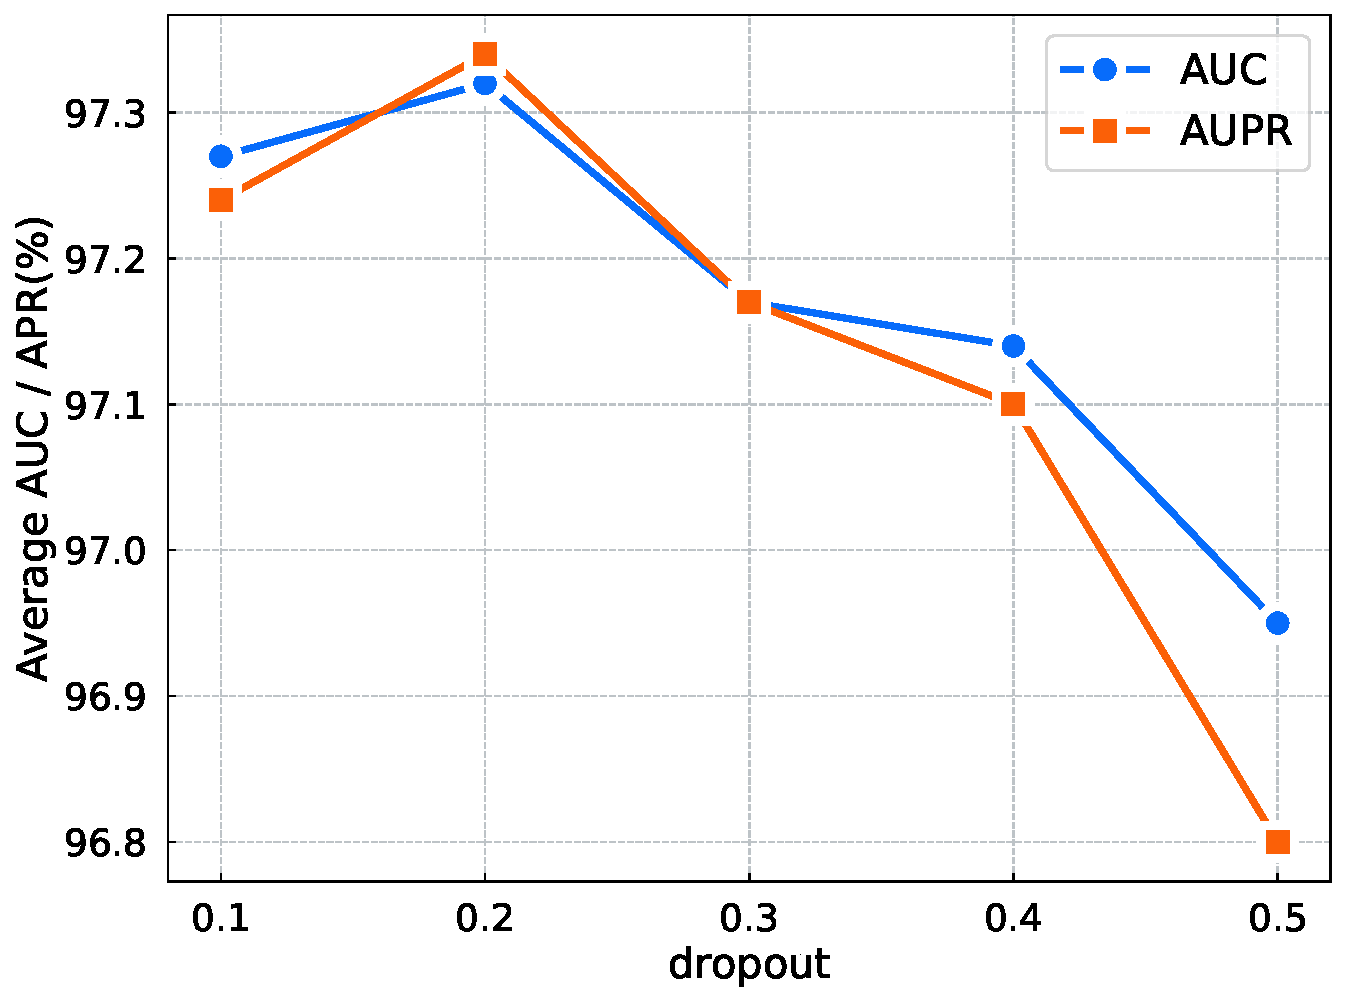
\includegraphics[width=3in]{dropout.pdf} &
		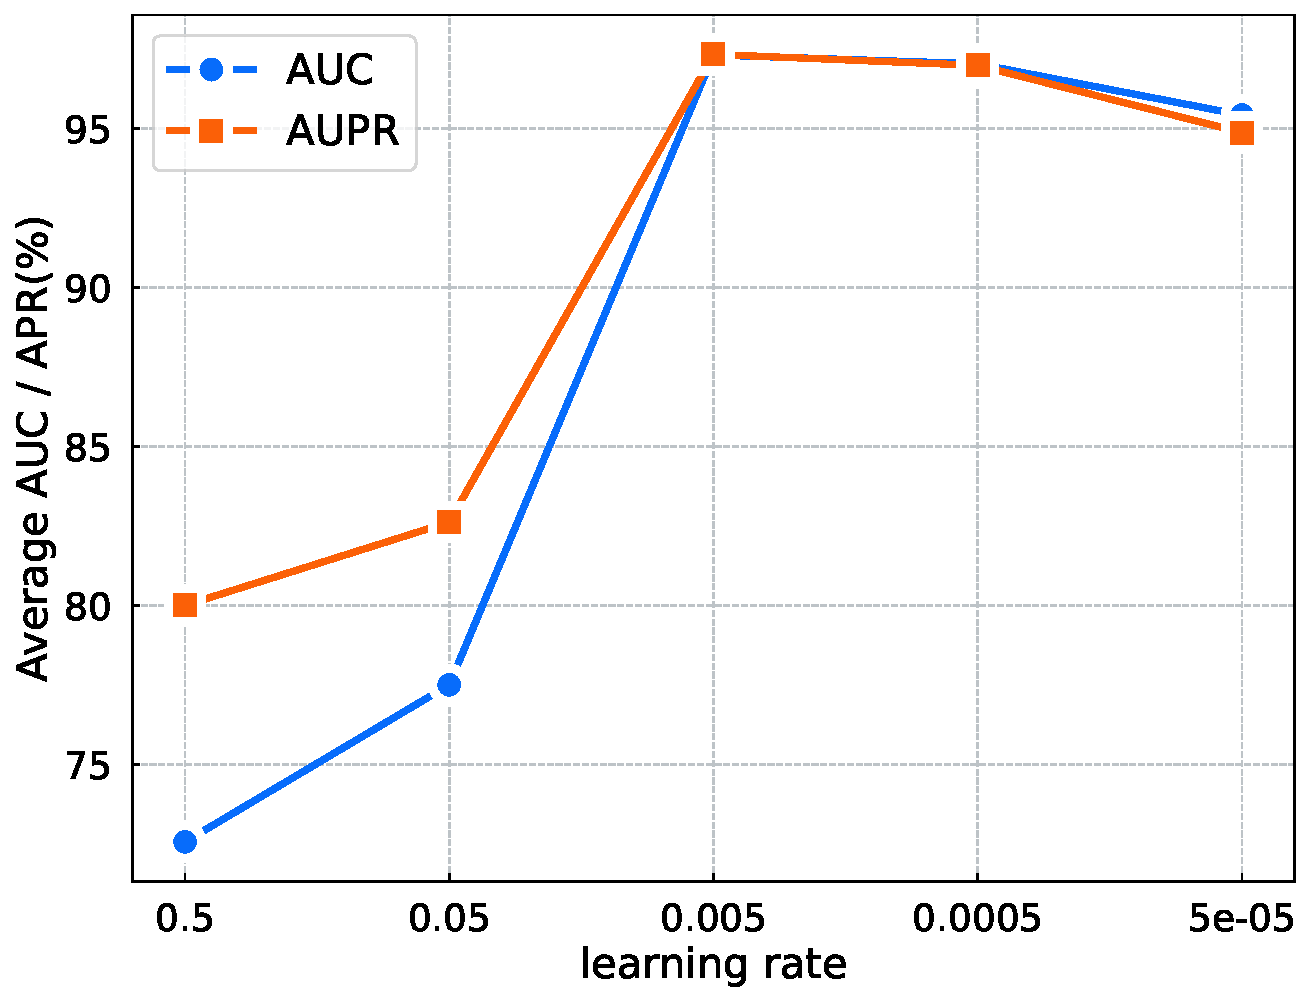
\includegraphics[width=3in]{learning_rate.pdf} \\
	\end{tabular}
	\vspace{-1mm} %调整纵向距离
	
	\caption{Effect of parameters in AGKphormer model on average AUC and AUPR. Top row: GCN layers (left), output dimension (right). Bottom row: dropout (left), learning rate (right).}
	\vspace{-3mm} %调整纵向距离
	\label{parameter}
\end{figure*}


After constructing our AGKphormer model, we employed evaluation metrics to measure its performance. To thoroughly assess the model's effectiveness and select the optimal configuration, we utilized the efficient and practical machine learning method of five-fold cross-validation\cite{wong2017dependency}. This approach fully leverages the dataset by evaluating the model's performance on different subsets, aiding us in more accurately selecting the best model or adjusting hyperparameters.

This method ensures that every sample has the opportunity to be used as test data, guaranteeing comprehensiveness and reliability in model assessment. It not only enhances the efficiency of data utilization but also helps us more precisely estimate the model's generalization ability.

To visually demonstrate the performance of our proposed model, we plotted the Receiver Operating Characteristic (ROC) curve. By visualizing the performance across different thresholds, the ROC curve helps assess the model's classification capability. Comparing the ROC curves of different models allows us to intuitively determine which model performs better. A larger area under the curve (AUC) value indicates better model performance.
To illustrate the relationship between precision and recall at different thresholds, we plotted the Precision-Recall curve (AUPR).
Additionally, we employed accuracy (Acc), precision (Pre), recall, and the F1 score as evaluation metrics.


%--------------------------------------------------------------------------------------------------------------

\subsection{Parameter experiment}

Following the modeling of the associations between metabolites and diseases using matrix completion and neural networks, we implemented the AGKphormer using the PyTorch deep learning framework. During model training, we fine-tuned several parameters. In the five-fold cross-validation, each fold was trained for 200 epochs, with hyperparameters such as the number of neural network layers, the number of multi-head attention heads, dropout rates, and learning rates all affecting the model's performance.

We used the method of holding variables constant to determine the optimal values for each parameter. We selected the number of GCN layers from the set \{1, 2, 3, 4\}, select the output dimension of the encoder from the set \{32, 64, 128, 256\}, the learning rate from the set \{0.009, 0.007, 0.005, 0.003, 0.001\}, and dropout from the set \{0.1, 0.2, 0.3, 0.4, 0.5\}. Fig.\ref{parameter} illustrates the impact of these parameters on AUC and AUPR, we can observe that the algorithm performs optimally and maintains a balance in terms of performance and complexity when there are two GCN layers,The output dimension is 128, a learning rate of 0.005, and a dropout rate of 0.2. 

Additionally, we have conducted experiments and filtered other parameters of model. In the calculation of disease semantic similarity, we set \(\Delta\) to 0.5, and the kernel bandwidth \({\omega}'\) in the Gaussian kernel similarity is set to 1. For matrix completion, we set the penalty parameter \(\rho\) of the ADMM algorithm to 1, and the threshold parameter \(\alpha\) to 0.01. In five-fold cross-validation, we chose Adam as the optimizer and selected the binary cross-entropy function. For the selection of our model parameters, see Tab.\ref{parameter_t}.


\begin{table}[]
	\centering
	\vspace{-1mm} %调整纵向距离
	\caption{The parameters of AGKphormer}
	\begin{tabular}{lll}
		\toprule
		\textbf{Structure} & \textbf{Parameters} & \textbf{value} \\
		\midrule
		ADMM & \(\rho\) & 1.0 \\
		& \(\alpha\) & 0.01 \\
		& tol & 1e-4 \\
		
		Encode & GCN layers & 2 \\
		& Output dim of Layer1 & 64 \\
		& Output dim of Layer2 & 64 \\
		& The heads of MHA & 1 \\
		& Output dim of MHA & 64 \\
		& dropout & 0.2 \\
		& learning rate & 0.005 \\
		& Loss function & binary cross entropy \\
		& Optimizer & Adam \\
		& Epoch & 200 \\
		& init scale & 0.1 \\
		& grid min & -2 \\
		& grid max & 2 \\
		& num grids & 8 \\
		& base activation & silu \\
		
		Decode & gain & 1.414\\
		
		\bottomrule
		\vspace{-5mm} %调整纵向距离
		\label{parameter_t}
	\end{tabular}
\end{table}

\begin{figure*}[htbp]
	\centering
	\vspace{-1mm} % 调整纵向距离
	\begin{tabular}{cc}
		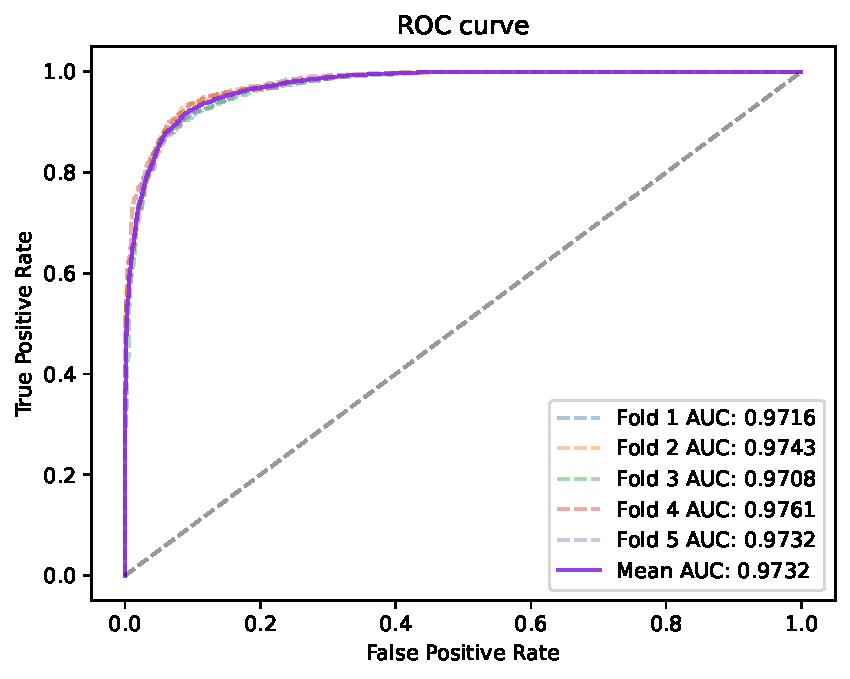
\includegraphics[width=3in]{test_auc.pdf} & 
		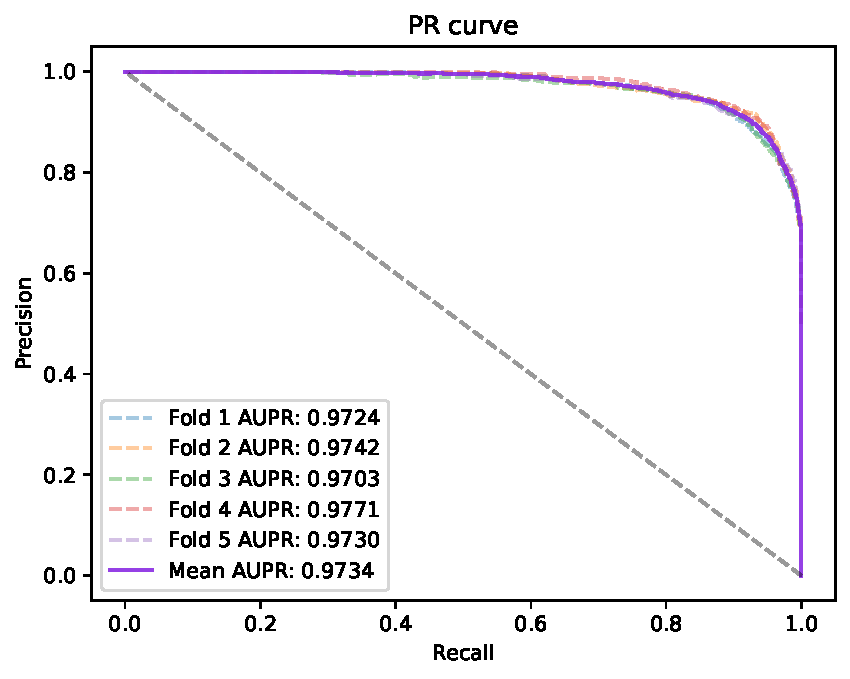
\includegraphics[width=3in]{test_prc.pdf} \\
	\end{tabular}
	\vspace{-2mm} % 调整纵向距离
	\caption{Performance curves of the AGKphormer model under five-fold cross-validation. Left: ROC curves. Right: PR curves.}
	\vspace{-3mm} %调整纵向距离
	\label{test}
\end{figure*}



After parameter tuning, the optimal results were achieved, and in Tab.\ref{table2} and Fig.\ref{test}, we provide feedback on the comprehensive performance of the model. From Table II, it can be seen that under the optimal parameters, the average Acc, Pre, Recall, and F1 scores of the AGKphormer model reached 91.68\%, 90.91\%, 92.61\%, and 91.75\%, respectively. In addition, as shown in Figure.4, the average AUC of the AGKphormer model's five-fold cross-validation reached 97.43\%, which is the average of 97.37\%, 97.44\%, 97.50\%, 97.51\%, and 97.31\%. As shown in Figure.4, the average AUPR of the AGKphormer model's five-fold cross-validation reached 97.40\%, which is the average of 97.24\%, 97.30\%, 97.55\%, 97.58\%, and 97.32\%.
\begin{table}[htbp]
	\centering
	\vspace{-1mm} %调整纵向距离
	\caption{The parameters of AGKphormer}
	\begin{tabular}{lllll}
		\toprule
		Fold & Acc(\%) & Pre(\%) & Recall(\%) &F1(\%) \\
		\midrule
		1 & 91.02 & 91.85 & 90.02 & 90.93 \\
		2 & 92.33 & 91.55 & 93.28 & 92.40 \\ %acc: 0.9233 Val Pre: 0.9155 Val Recall: 0.9328 Val F1: 0.9240 
		3 & 91.07 & 90.39 & 91.91 & 91.15 \\ %acc: 0.9107 Val Pre: 0.9039 Val Recall: 0.9191 Val F1: 0.9115
		4 & 91.96 & 90.56 & 93.70 & 92.10 \\ %acc: 0.9196 Val Pre: 0.9056 Val Recall: 0.9370 Val F1: 0.9210
		5 & 91.20 & 89.39 & 93.51 & 91.40 \\ %acc: 0.9120 Val Pre: 0.8939 Val Recall: 0.9351 Val F1: 0.9140
		Mean & 91.52 & 90.75 & 92.48 & 91.62 \\
		
		\bottomrule
		\vspace{-7mm} %调整纵向距离
		\label{table2}
	\end{tabular}
\end{table}

This means that our model has good accuracy, strong generalization ability, and superior interpretability.The outstanding performance of the AGKphormer model can be attributed to the following reasons: firstly, we use the ADMM optimization algorithm to solve the heterogeneous matrix with minimum nuclear norm to complete the association matrix, making the original association matrix no longer sparse, which is more conducive to our more precise predictions. Secondly, we combine GCN with the introduced FastKAN multi-head attention to extract features from the heterogeneous network, learning neighborhood features while further learning global features. In addition, the introduction of FastKAN has improved the model's interpretability and also demonstrated the model's good generalization ability. Through training the model and parameter tuning, the best performance is achieved.



%--------------------------------------------------------------------------------------------------------------

\begin{figure*}[htbp]
	\centering
	\vspace{-3mm} % 调整纵向距离
	\begin{tabular}{cc}
		\includegraphics[width=3in]{Ablatioin_AUC.pdf} & 
		\includegraphics[width=3in]{Ablatioin_AUPR.pdf} \\
	\end{tabular}
	\vspace{-1mm} % 调整纵向距离
	
	\caption{Average AUPR and AUC of AGKphormer and ablation models on five-fold cross-validation.}
	\vspace{-1mm} %调整纵向距离
	\label{Ablation}
\end{figure*}

\begin{table*}[!htbp]
	\centering
	\vspace{-2mm} %调整纵向距离
	\caption{Performance comparison between the AGKphormer and five benchmark methods on datasets 1 and 2}
	\begin{tabular}{@{}l
			*{2}{>{\centering\arraybackslash}p{1.5cm}}
			*{6}{>{\centering\arraybackslash}p{1.2cm}}@{}}
		\toprule
		\multirow{2}{*}{Method} & 
		\multicolumn{4}{c}{Dataset 1} & 
		\multicolumn{4}{c}{Dataset 2} \\
		\cmidrule(lr){2-5} \cmidrule(lr){6-9}
		& {Acc(\%)} & {Pre(\%)} & {Recall(\%)} & {F1(\%)} & {Acc(\%)} & {Pre(\%)} & {Recall(\%)} & {F1(\%)} \\
		\midrule
		AGKphormer  & \textbf{91.52} & \textbf{90.75} & \textbf{92.48} & \textbf{91.60} & \textbf{91.51} & $\underline{90.02}$ & \textbf{93.39} & \textbf{91.66} \\
		MDBIBW     & 80.43 & 79.02 & 82.90 & 80.89 & 78.10 & 77.20 & 79.82 & 78.46 \\
		DWRF       & 88.01 & $\underline{90.27}$ & 85.34 & 87.74 & 87.08 & 87.08 & 89.88 & 86.83 \\
		DeepDRM    & 89.20 & 87.59 & 90.21 & 89.69 & 89.50 & 87.75 & 90.60 & 89.14 \\
		GCNAT      & 88.22 & 87.70 & 89.14 & 88.34 & 90.19 & \textbf{91.93} & 89.20 & $\underline{91.00}$ \\
		MDA-AENMF  & $\underline{90.76}$ & 89.95 & $\underline{91.87}$ & $\underline{90.86}$ & $\underline{90.43}$ & 88.74 & $\underline{92.65}$ & 90.64 \\
		\bottomrule
	\end{tabular}
	\vspace{-3mm} %调整纵向距离
	\label{tablep}
\end{table*}



\subsection{Ablation experiments}
We performed an ablation study on our model's modules to determine the contribution of each submodule. While keeping other modules unchanged, we removed one module at a time and conducted experiments on the same dataset.
\begin{itemize}
	\item Del-ADMM: We do not use the completed association matrix; instead, we utilize the original sparse matrix.
	
	\item Del-GCN: Remove the GCN layer, leaving only a simplified encoder with multi-head attention and FastKAN.
	
	\item Del-MHA: A simplified encoder that retains only the GCN and FastKAN components.
	
	\item Del-FastKAN: Remove FastKAN to obtain an encoder composed of GCN layers and multi-head attention.
	
\end{itemize}

As shown in Fig.\ref{Ablation}, the AGKphormer model's performance in the ablation study is demonstrated with the impact of different components on AUC and AUPR. By progressively removing various components from the model, we can assess the contribution of each part to the overall performance. The results indicate that the AUC and AUPR values of the AGKphormer model reach 97.32\% and 97.34\%, respectively, which are higher than those of other ablation models. When different components are removed, the model's performance decreases. Del-ADMM's AUC and AUPR values drop to 95.77\% and 95.13\%, suggesting that the completion of the association matrix can improve model accuracy. Del-GCN further reduces the AUC and AUPR values to 94.03\% and 94.06\%, highlighting the importance of the GCN layer in feature extraction. The AUC and AUPR values of Del-MHA are 95.08\% and 93.65\%, respectively, indicating that the multi-head attention mechanism is beneficial for learning long-range dependency features. Del-FastKAN's AUC and AUPR values are 96.39\% and 95.84\%, with a decrease in performance, implying that FastKAN can accelerate model convergence and enhance accuracy.

Overall, the ablation study results emphasize the significance of each component in the AGKphormer model. Through this analysis, we can better understand the model's internal working mechanisms and provide guidance for future model optimization.

\begin{figure*}[htbp]
	\centering
	\vspace{-1mm} % 调整纵向距离
	\begin{tabular}{cc}
		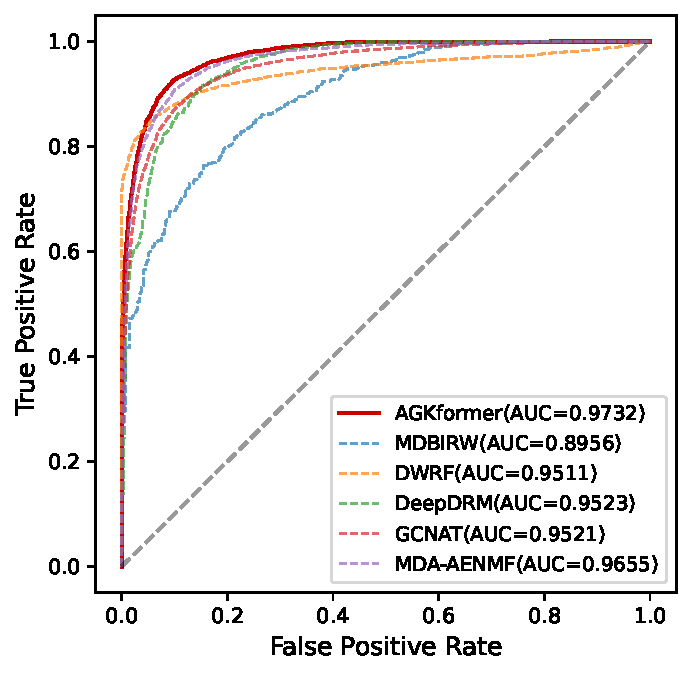
\includegraphics[width=3in]{Comparative_experiment_ROC_1.pdf} & 
		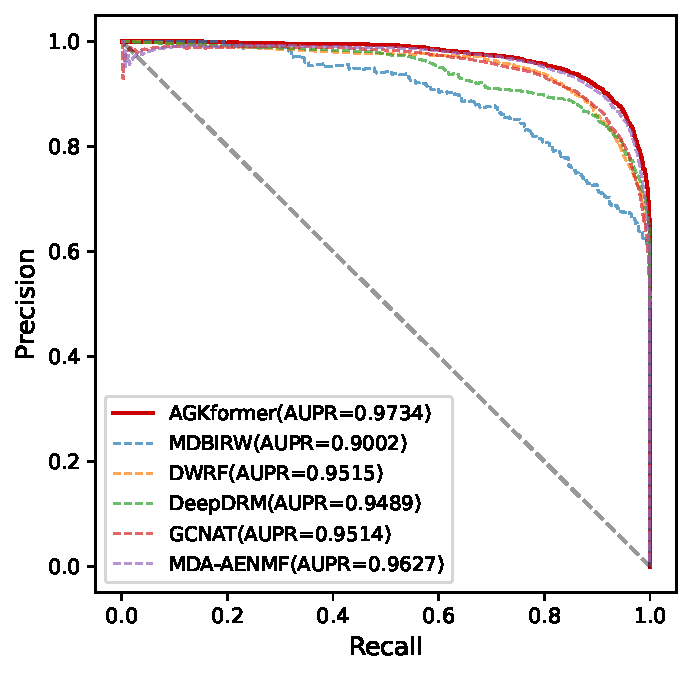
\includegraphics[width=3in]{Comparative_experiment_PR_1.pdf} \\
	\end{tabular}
	\vspace{-2mm} % 调整纵向距离
	
	\caption{Performance comparison of AGKphormer and benchmark methods under five-fold cross-validation. Left: ROC curves. Right: PR curves.}
	\vspace{-3mm} %调整纵向距离
	\label{comparison_AUCPR}
\end{figure*}

\subsection{Comparative Experiment}
\subsubsection{Comparison with benchmark approaches}
To intuitively demonstrate the advantages of AGKphormer, we compared it with the association prediction methods that have emerged in the field of bioinformatics in recent years, and conducted tests and comparative analyses on the same datasets.
\begin{itemize}
	\item Bi-randomwalks (MDBIRW)\cite{lei2019prediction} predicts disease-related metabolites by reconstructing disease similarity networks and metabolite functional similarity networks, and then performing a double random walk algorithm on these networks.
	
	\item DWRF\cite{tie2021metabolite} integrates different similarity metrics for diseases and metabolites, applies DeepWalk for feature extraction, and then uses random forests to predict the potential associations between metabolites and diseases.
	
	\item Deep-DRM\cite{zhao2021deep} constructs networks of metabolites and diseases, uses GCN to encode features, applies PCA for dimensionality reduction, and then identifies related metabolites through a deep neural network.
	
	\item GCNAT\cite{sun2022deep} constructs a heterogeneous network, encodes features with GCN, integrates embeddings using a graph attention layer, and decodes and scores to predict disease-related metabolites.
	
	\item MDA-AENMF\cite{gao2023predicting} integrates various similarity networks and uses autoencoders and matrix factorization to extract features, merging them into a comprehensive feature vector for each metabolite-disease pair to predict potential associations. 
	
\end{itemize}

AGKphormer was compared with the aforementioned algorithms, and the results are shown in Tab.\ref{tablep}. Bold values indicate the best results, while underlined values represent the second-best results. AGKphormer demonstrates significant advantages across all key metrics on both Dataset 1 and Dataset 2. Specifically, on Dataset 1, AGKphormer achieved improvements of 0.76\%, 0.61\%, and 0.74\% in Accuracy (Acc), Recall, and F1-score respectively compared to the second-ranked MDA-AENMF. In terms of Precision (Pre), it outperformed the second-best model DWRF by 0.48\%. Moreover, as significantly shown in Fig.\ref{comparison_AUCPR}, AGKphormer's ROC and PR curves are superior to those of the other five baseline methods. AGKphormer has the largest area under the ROC curve, with an AUC value of 97.32\%, which is 7.76\%, 2.21\%, 2.09\%, 2.11\%, and 0.77\% higher than MDBIRW, DWRF, DeepDRM, GCNAT, and MDA-AENMF, respectively, indicating that our model performs quite ideally. Moreover, AGKphormer achieved the highest Area Under the Precision-Recall Curve (AUPR) of 97.34\%, demonstrating superior performance in positive sample identification. On Dataset 2, AGKphormer maintained this outstanding performance, securing top rankings with AUC and AUPR scores of 97.03\% and 96.34\% respectively. This indicates that AGKphormer can maintain high accuracy while better identifying all positive samples, highlighting its exceptional performance and potential value in practical applications.



The aforementioned methods all utilize sparse bipartite heterogeneous networks. Our proposed method is based on enhanced metabolite-disease associations. This matrix, along with the similarity networks, is input into a GCN for feature extraction. A transformer is used to learn global dependencies, followed by further nonlinear transformations through a FastKAN feedforward network, and finally, the associations are decoded to obtain the final relationships. This approach not only improves accuracy but also enhances the model's interpretability.

\subsubsection{Comparative Analysis of Matrix completion}
In this study, we propose a nuclear norm minimization-based correlation matrix completion method to address the challenges of sparsity and low-rank characteristics in metabolic-disease association networks. To validate its advantages over traditional link enhancement methods, we conducted five-fold cross-validation comparative experiments under fixed random seeds and hardware configurations, comparing the    nuclear norm optimization framework with classical approaches such as matrix factorization (MF) and neighborhood propagation (NP).

As shown in the radar chart of Fig.\ref{ADMM}, the nuclear norm minimization method significantly outperforms traditional methods in key metrics including AUROC and AUPR, while demonstrating computational efficiency comparable to matrix factorization approaches. The experimental results indicate that the ADMM-based nuclear norm minimization framework exhibits both robustness and scalability in sparse biological network completion tasks, providing high-confidence association prior knowledge for subsequent predictive models.
\begin{figure}[]
	\centering
	\vspace{-3mm} %调整纵向距离
	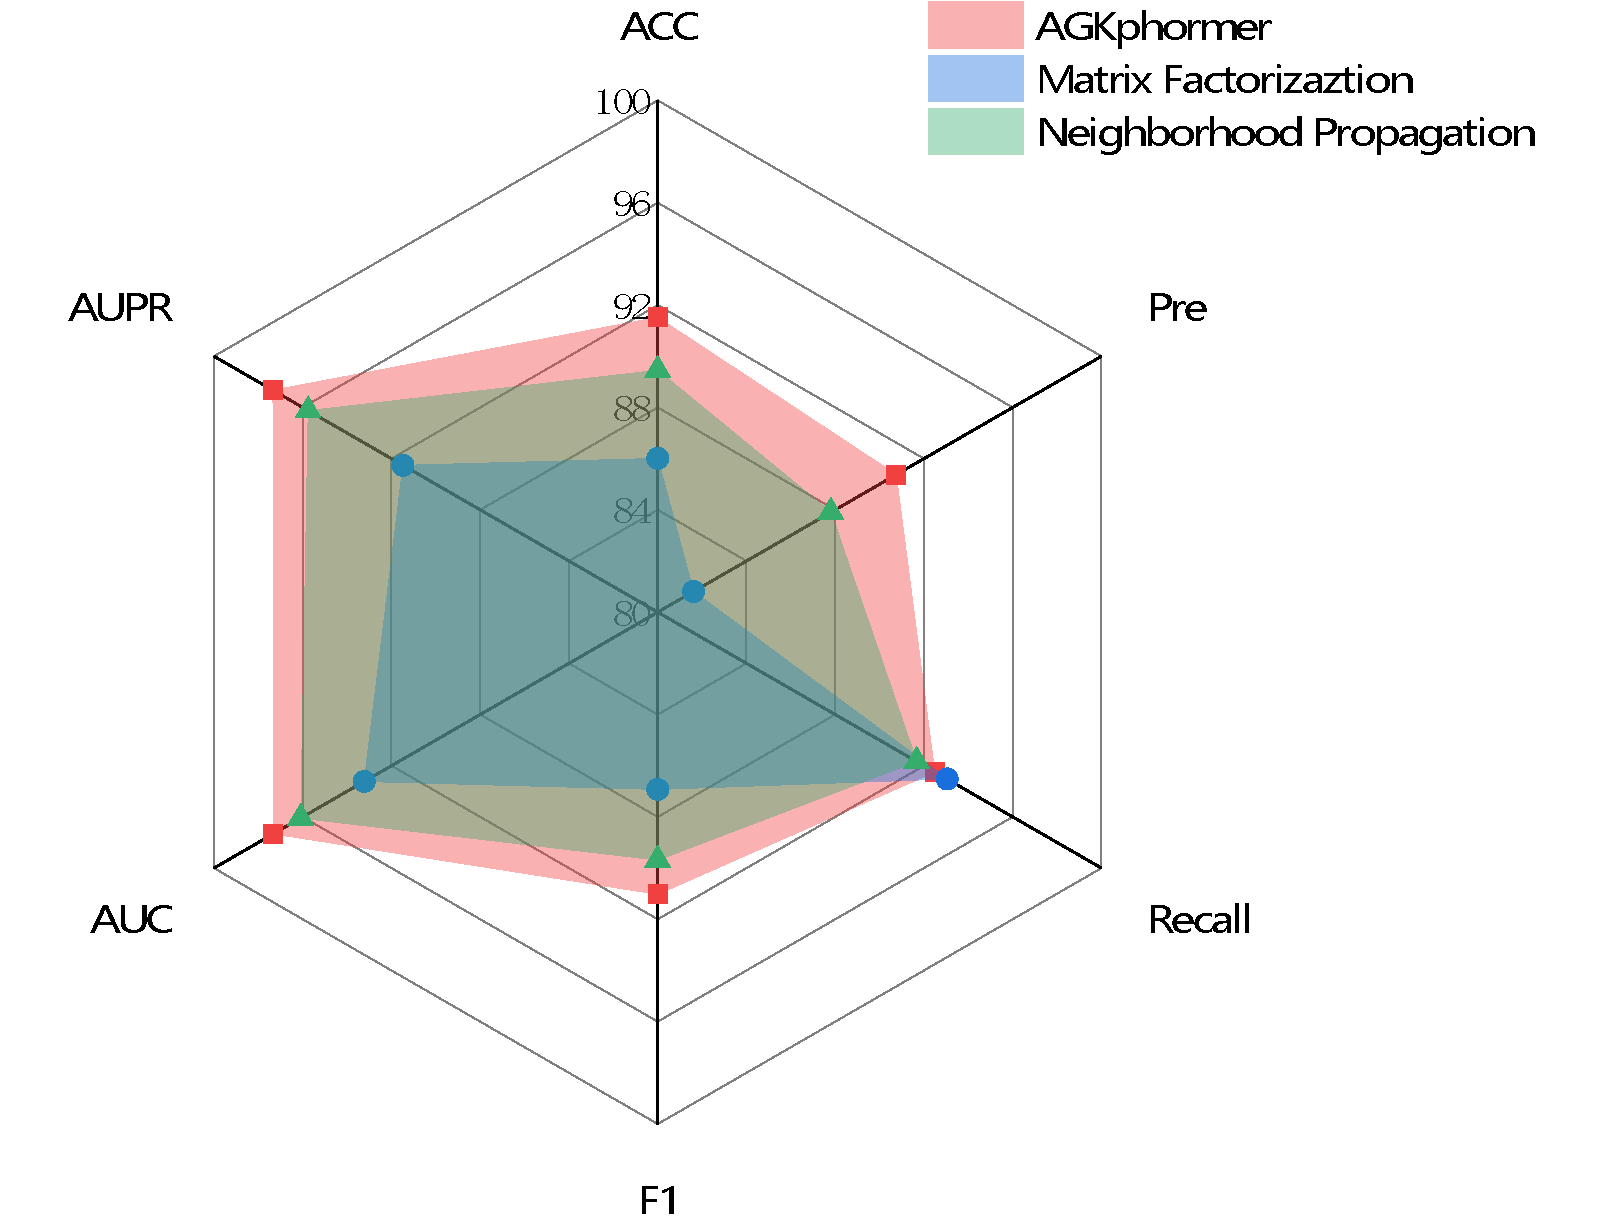
\includegraphics[width=2.8in]{ADMM.pdf}
	\vspace{0mm} %调整纵向距离
	\caption{Performance comparison of nuclear norm minimization with two classical matrix completion methods.}
	\vspace{-3mm} %调整纵向距离
	\label{ADMM}
\end{figure}
\subsubsection{Comparative Analysis of FastKAN}
In our study, we propose an enhanced FastKAN architecture that enhances non-linear expressive power and provides more comprehensive feature representations for subsequent decoding. To validate its superior performance compared to traditional MLP with fixed activation functions (e.g., ReLU) and standard kernel methods, we conducted comparative experiments against conventional MLP and Support Vector Machine (SVM) approaches, with all methods adopting default parameter configurations.

As shown in Fig.\ref{FastKAN}, the FastKAN architecture significantly outperforms other architectures in terms of Acc, Pre, Recall, F1, AUC, and AUPR. This superior performance is primarily attributed to the following aspects: FastKAN adaptively captures node features by placing activation functions at the network edges and employing learnable radial basis terms; secondly, it ensures smoothness constraints during feature propagation through the use of third-order spline bases. This enables it to achieve more accurate function fitting in both low-dimensional and high-dimensional tasks.

\begin{figure}[]
	\centering
	\vspace{-3mm} %调整纵向距离
	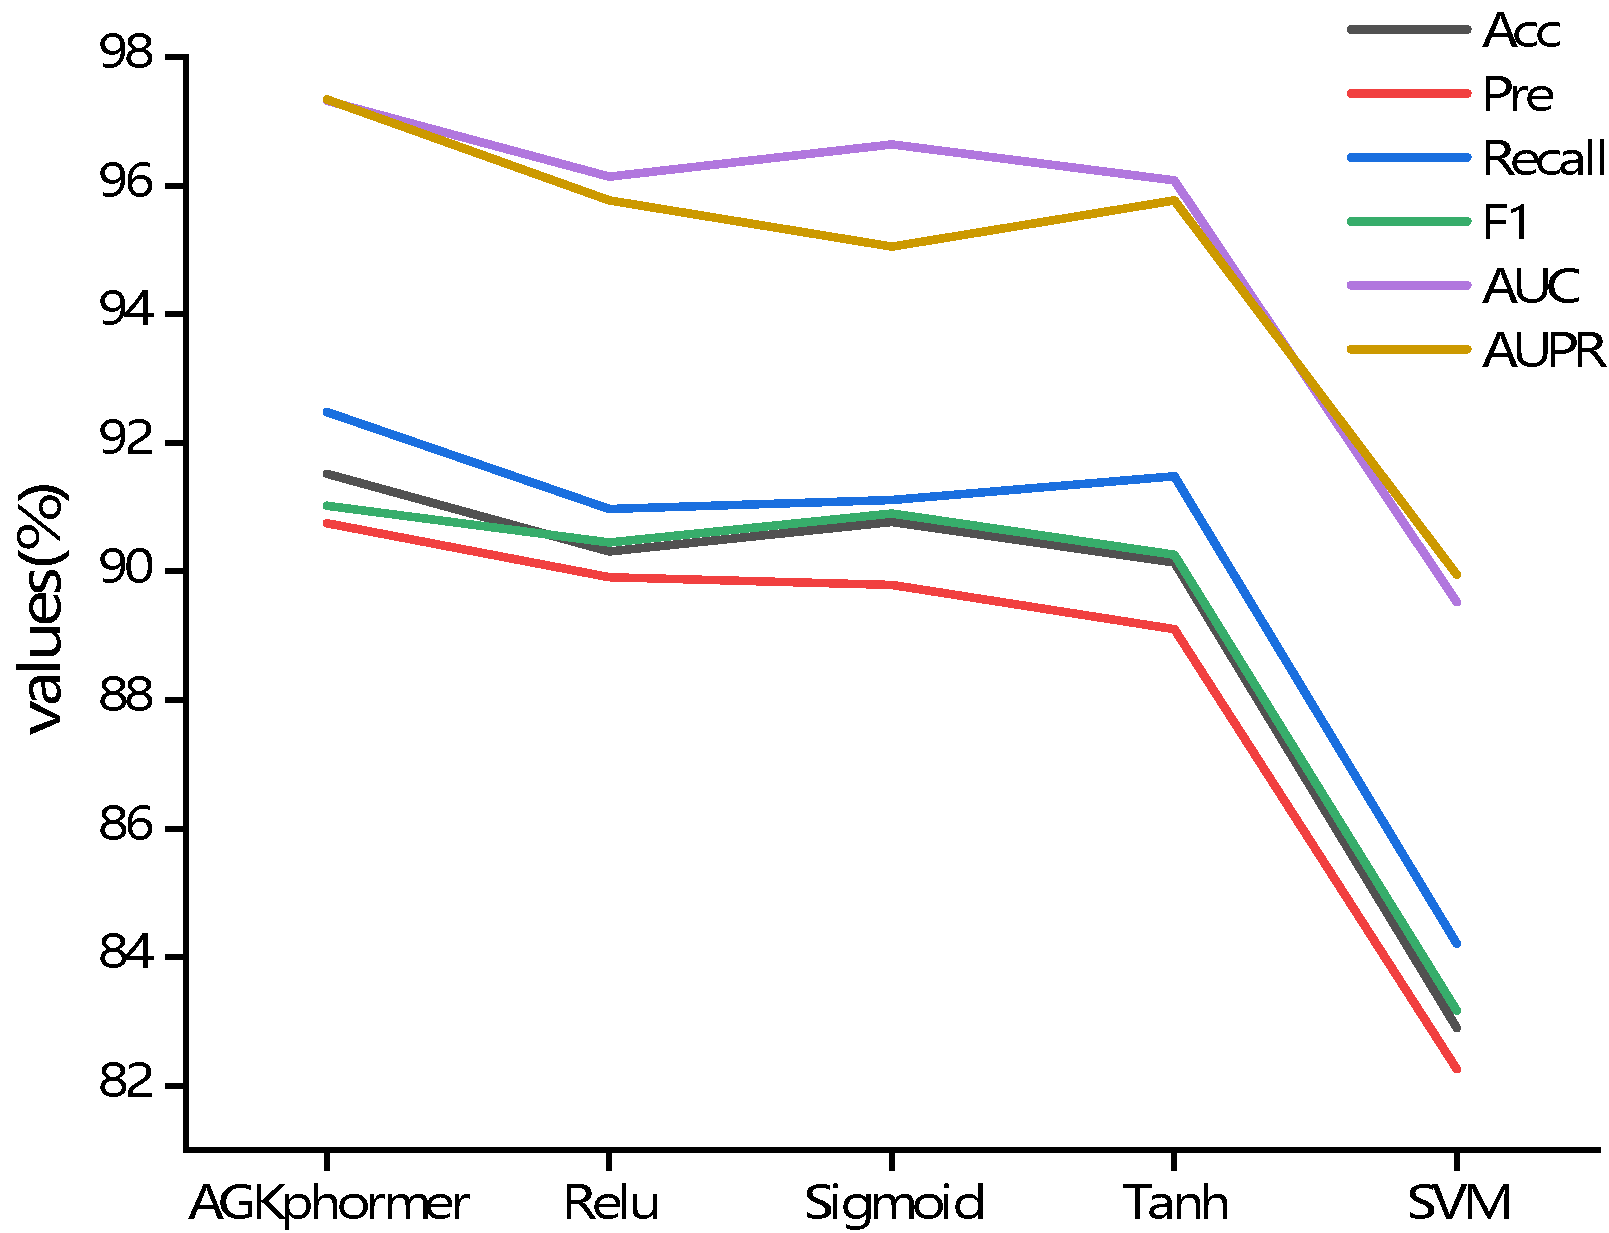
\includegraphics[width=2.8in]{kan.pdf}
	\vspace{0mm} %调整纵向距离
	\caption{Performance comparison between FastKAN and four classic machine learning models.}
	\vspace{-3mm} %调整纵向距离
	\label{FastKAN}
\end{figure}

\subsection{Case study}
To evaluate the practical effectiveness of the AGKphormer model, we conducted an in-depth analysis of two complex diseases-Alzheimer's disease and Crohn's disease. Specifically, we selected Alzheimer's disease and Crohn's disease along with all associated metabolites as the positive samples for the test set, and randomly selected an equal number of unknown associations as the negative samples. We then used all samples outside of these diseases as the training set. Ultimately, we obtained association scores between specific diseases and metabolites, ranked them, and identified the top 15 associated metabolites. To verify the accuracy of these predictions, we conducted detailed literature searches and data analysis using the HMDB and NCBI databases.


\begin{table}[h]
	\centering
	\vspace{-3mm} %调整纵向距离
	\caption{Predicted results of top 15 metabolites associated with Alzheimer's disease}
	\begin{tabular}{llll}
		\toprule
		Rank & Metabolite & Probability & PMID \\ 
		\midrule
		
		1 &	Creatinine &	0.9998  &	23857558 \\
		2 &	alpha-D-Glucose &	0.9998 & 	9693263\\
		3 &	D-Glucose &	0.9992 & 	9693263 \\
		4 &	Hypoxanthine &	0.9989 & 	23857558 \\
		5 &	Homocysteine &	0.9983  &	21474939\\
		6 &	Adenine &	0.9959  &	23857558\\
		7 &	Chloroform &	0.9951 & 	None \\
		8 &	L-Alanine &	0.9921 &	23857558 \\
		9 &	Hexadecanedioic acid &	0.9906 & 	None\\
		10 &	Dopamine &	0.9902 &	17031479 \\
		11 &	Substance P &	0.9899 &	11314776\\
		12 &	Mannitol &	0.9871 &	8595727 \\
		13 &	L-Arginine &	0.9866 &	17031479 \\
		14 &	L-Proline &	0.9855 &	17031479 \\
		15 &	Choline &	0.9850 &	15465626\\
		
		\bottomrule
		\vspace{-5mm} %调整纵向距离
		\label{table3}
	\end{tabular}
\end{table}

\begin{table}[h]
	\centering
	\vspace{-3mm} %调整纵向距离
	\caption{Predicted results of top 15 metabolites associated with Crohn's disease}
	\begin{tabular}{llll}
		\toprule
		Rank & Metabolite & Probability & PMID \\ 
		\midrule
		
		1&	L-Serine&	0.9629&	27609529 \\
		2&	Glycine&	0.9566&	25598765 \\
		3&	Isobutyric acid&0.9506& 24811995 \\
		4&	L-Glutamine&	0.9422&	27609529 \\
		5&	D-Aspartic acid&	0.9405&	17269711 \\
		6&	D-Glutamic acid&	0.9382&	17269711 \\
		7&	L-Alanine&	0.9358&	17269711 \\
		8&	L-Tyrosine&	0.9340&	25598765 \\
		9&	Hydrocinnamic acid&	0.9337&	28842642 \\
		10&	Acetic acid&	0.9318&	17269711 \\
		11&	beta-Alanine&	0.9293&	28842642 \\
		12&	Creatine&	0.9276&	27609529 \\
		13&	L-Lysine&	0.9228&	17269711 \\
		14&	L-Threonine&	0.9210&	17269711 \\
		15&	Deoxyuridine&	0.9186&	27609529 \\
		
		\bottomrule
		\vspace{-5mm} %调整纵向距离
		\label{table4}
	\end{tabular}
\end{table}

Alzheimer's disease\cite{blennow2006alzheimer} is a common neurodegenerative disorder primarily affecting the elderly, impacting memory, cognitive abilities, and responsiveness. As a prevalent condition, there is currently no effective treatment; management mainly focuses on alleviating symptoms and enhancing quality of life. The exact cause remains unclear, but it is associated with various genetic and environmental factors.
Currently, some researchers have found that the levels of metabolites in patients differ from those in healthy individuals \cite{chen2013decoding}. They are trying to study and diagnose Alzheimer's disease in advance based on metabolites\cite{wilkins2018application}. In recent years, the emergence of certain algorithms has provided us with more efficient methods. Tab.\ref{table3} lists the top 15 metabolites predicted by our proposed AGKphormer model to be highly related to Alzheimer's disease, and 13 of them have been verified. Our model predicts that Creatine\cite{tsuruoka2013capillary}, alpha-D-Glucose, and D-Glucose\cite{redjems1998abnormal} are the three most related metabolites to the disease, with probability values of 0.9998, 0.9998, and 0.9992, respectively. Additionally, the verification of other metabolites can be found in the reference literaturesuch as L-Alanine, Hypoxanthine, and L-Phenylalanine. These high probability values indicate a strong association between these metabolites and Alzheimer's disease. In addition, our model also predicts several other metabolites, such as Chloroform and Hexadecanedioic acid, which also show significant relevance to Alzheimer's disease.


\begin{figure*}[]
	\centering
	\vspace{-3mm} %调整纵向距离
	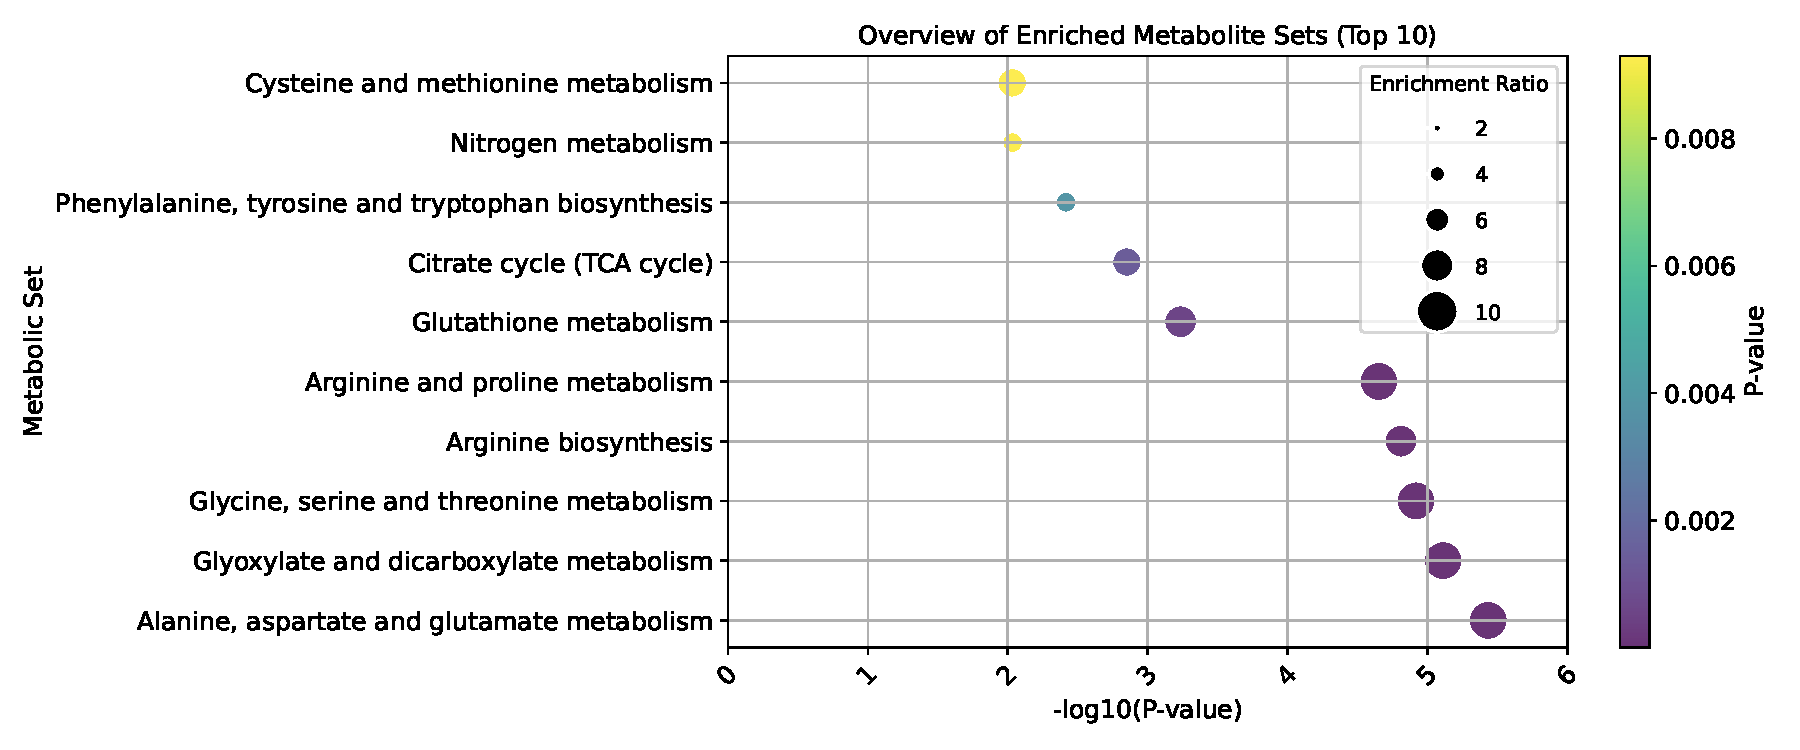
\includegraphics[width=15cm]{enriched_analysis.pdf}
	\vspace{-3mm} %调整纵向距离
	\caption{Performance comparison between the proposed AGKphormer model and five benchmark methods based on five-fold cross-validation.}
	\vspace{-3mm} %调整纵向距离
	\label{Enrichment Analysis}
\end{figure*}

Crohn's disease\cite{shanahan2002crohn} is a chronic inflammatory bowel disease that significantly affects the digestive tract, but it most commonly impacts the terminal ileum and the colon. This disease typically causes chronic inflammation and ulceration of the intestines, leading to a range of discomforts and symptoms.
Tab. \ref{table4} presents the top 15 metabolites predicted to be highly associated with Crohn's disease, predicting that L-Serine\cite{kolho2017faecal}, Glycine\cite{bjerrum2015metabonomics}, and Isobutyric acid\cite{de2015faecal} are the three metabolites most closely associated with the disease, with probability values of 0.9629, 0.9565, and 0.9506, respectively. Additionally, the verification of other metabolites can be found in the reference literature. These high probability values further confirm the potential links between these metabolites and Crohn's disease. The model also predicted other metabolites related to Crohn's disease, such as L-Glutamine, D-Aspartic acid, and D-Glucuronic acid.


\subsection{Enrichment Analysis}

Metabolite pathway enrichment analysis is a bioinformatics method used to determine whether differentially expressed metabolites in specific biological samples are significantly enriched in particular metabolic pathways. This can help verify whether the metabolites predicted by the AGKphormer model are involved in important processes of known metabolic pathways. First, we selected the top 50 metabolites predicted by AGKphormer to be associated with Alzheimer's disease. Next, we annotated them by comparing them with the KEGG database\cite{kanehisa10new}. Then, we identified their positions in metabolic pathways and calculated the significance of enrichment. Finally, we used the tool MetaboAnalyst\cite{pang2024metaboanalyst} for visualization to reveal the functions and roles of these metabolites in biological processes.

Fig.\ref{Enrichment Analysis} displays the results of metabolite pathway enrichment analysis, listing the top 10 significantly enriched metabolic pathways, such as "Alanine, aspartate and glutamate metabolism." The x-axis represents the enrichment ratio, the y-axis lists the pathway names, and the color or z-axis indicates the negative logarithm of the P-value, with higher values signifying greater significance of enrichment.This supports the accuracy of the AGKphormer model and helps to better understand the mechanisms of Alzheimer's disease, providing potential for the development of targeted therapeutic strategies.





\section{AGKphormer web server}
A web server that implements AGKphormer is freely available at  
\href{https://lutgraphgroup.github.io/agkphormer.github.io/}  
{\texttt{agkphormer}}.  
When using AGKphormer, the user needs to input a metabolite name. The user then clicks the search button to view the prediction results. The results include the diseases associated with the metabolite and the association scores.


\section{Conclusions}\label{sec6}
Metabolic disease association research aims to explore the potential connections between them to identify biomarkers and therapeutic targets, which is crucial for disease diagnosis, treatment, and prevention. By analyzing changes in metabolites, scientists can uncover disease mechanisms and provide a basis for developing new therapies. Traditional biological experiments are inefficient. The accuracy and interpretability of computational methods still need improvement, necessitating new algorithms to address the shortcomings of current approaches. Our proposed AGKphormer uses a completed association matrix and deep learning to learn features, achieving more accurate predictions. First, we utilize an ADMM optimization algorithm based on similarity networks of metabolites and diseases to complete the known metabolite-disease association matrix, making the original matrix less sparse. Then, we employ GCN and multi-head attention for feature learning, capturing long-range dependencies more effectively. Finally, by scoring the final embeddings, we obtain the predicted results. Through five-fold cross-validation, compared with baseline methods, AGKphormer achieved the best results with AUC(97.32\%) and AUPR(97.34\%). Additionally, we conducted ablation experiments on our model's modules, verifying the contribution of each module and the overall robustness. Lastly, we conducted case studies on Alzheimer's disease and Crohn's disease, and the results consistently show that our model is precise in predicting disease and metabolite associations.

The AGKphormer model shows improved performance compared to previous models.First, we use the ADMM algorithm to solve the minimum nuclear norm to complete the original sparse matrix, enhancing the model's predictive accuracy. Second, we employ GCN to extract neighborhood features of nodes and learn the underlying patterns of the data. Third, while learning neighborhood features, we use multi-head attention to capture long-distance dependencies, compensating for the shortcomings of GCN. Additionally, we are the first to use FastKAN in disease prediction, which, compared to traditional neural networks, improves the model's interpretability.


\section*{Data availability statement}
The codes and data sets are available online at \url{https://github.com/LUTGraphGroup/AGKphormer_ZhangJian.git}.


\section*{Funding}
This work was supported by the Gansu Province Key R\&D  Plan with No.24YFFA023, Gansu Province Industrial Support Plan with No.2023CYZC-25,  and  Natural Science Foundation of Gansu Province with No.23JRRA770.   

\section*{Ethics declarations}
This study was conducted in compliance with the ethical standards and guidelines for research that does not involve human or animal subjects. All authors have reviewed and approved this manuscript for publication.


\bibliographystyle{unsrt}
\bibliography{references}

\end{document}

